% Options for packages loaded elsewhere
\PassOptionsToPackage{unicode}{hyperref}
\PassOptionsToPackage{hyphens}{url}
%
\documentclass[
]{book}
\usepackage{amsmath,amssymb}
\usepackage{lmodern}
\usepackage{iftex}
\ifPDFTeX
  \usepackage[T1]{fontenc}
  \usepackage[utf8]{inputenc}
  \usepackage{textcomp} % provide euro and other symbols
\else % if luatex or xetex
  \usepackage{unicode-math}
  \defaultfontfeatures{Scale=MatchLowercase}
  \defaultfontfeatures[\rmfamily]{Ligatures=TeX,Scale=1}
\fi
% Use upquote if available, for straight quotes in verbatim environments
\IfFileExists{upquote.sty}{\usepackage{upquote}}{}
\IfFileExists{microtype.sty}{% use microtype if available
  \usepackage[]{microtype}
  \UseMicrotypeSet[protrusion]{basicmath} % disable protrusion for tt fonts
}{}
\makeatletter
\@ifundefined{KOMAClassName}{% if non-KOMA class
  \IfFileExists{parskip.sty}{%
    \usepackage{parskip}
  }{% else
    \setlength{\parindent}{0pt}
    \setlength{\parskip}{6pt plus 2pt minus 1pt}}
}{% if KOMA class
  \KOMAoptions{parskip=half}}
\makeatother
\usepackage{xcolor}
\usepackage{color}
\usepackage{fancyvrb}
\newcommand{\VerbBar}{|}
\newcommand{\VERB}{\Verb[commandchars=\\\{\}]}
\DefineVerbatimEnvironment{Highlighting}{Verbatim}{commandchars=\\\{\}}
% Add ',fontsize=\small' for more characters per line
\usepackage{framed}
\definecolor{shadecolor}{RGB}{248,248,248}
\newenvironment{Shaded}{\begin{snugshade}}{\end{snugshade}}
\newcommand{\AlertTok}[1]{\textcolor[rgb]{0.94,0.16,0.16}{#1}}
\newcommand{\AnnotationTok}[1]{\textcolor[rgb]{0.56,0.35,0.01}{\textbf{\textit{#1}}}}
\newcommand{\AttributeTok}[1]{\textcolor[rgb]{0.77,0.63,0.00}{#1}}
\newcommand{\BaseNTok}[1]{\textcolor[rgb]{0.00,0.00,0.81}{#1}}
\newcommand{\BuiltInTok}[1]{#1}
\newcommand{\CharTok}[1]{\textcolor[rgb]{0.31,0.60,0.02}{#1}}
\newcommand{\CommentTok}[1]{\textcolor[rgb]{0.56,0.35,0.01}{\textit{#1}}}
\newcommand{\CommentVarTok}[1]{\textcolor[rgb]{0.56,0.35,0.01}{\textbf{\textit{#1}}}}
\newcommand{\ConstantTok}[1]{\textcolor[rgb]{0.00,0.00,0.00}{#1}}
\newcommand{\ControlFlowTok}[1]{\textcolor[rgb]{0.13,0.29,0.53}{\textbf{#1}}}
\newcommand{\DataTypeTok}[1]{\textcolor[rgb]{0.13,0.29,0.53}{#1}}
\newcommand{\DecValTok}[1]{\textcolor[rgb]{0.00,0.00,0.81}{#1}}
\newcommand{\DocumentationTok}[1]{\textcolor[rgb]{0.56,0.35,0.01}{\textbf{\textit{#1}}}}
\newcommand{\ErrorTok}[1]{\textcolor[rgb]{0.64,0.00,0.00}{\textbf{#1}}}
\newcommand{\ExtensionTok}[1]{#1}
\newcommand{\FloatTok}[1]{\textcolor[rgb]{0.00,0.00,0.81}{#1}}
\newcommand{\FunctionTok}[1]{\textcolor[rgb]{0.00,0.00,0.00}{#1}}
\newcommand{\ImportTok}[1]{#1}
\newcommand{\InformationTok}[1]{\textcolor[rgb]{0.56,0.35,0.01}{\textbf{\textit{#1}}}}
\newcommand{\KeywordTok}[1]{\textcolor[rgb]{0.13,0.29,0.53}{\textbf{#1}}}
\newcommand{\NormalTok}[1]{#1}
\newcommand{\OperatorTok}[1]{\textcolor[rgb]{0.81,0.36,0.00}{\textbf{#1}}}
\newcommand{\OtherTok}[1]{\textcolor[rgb]{0.56,0.35,0.01}{#1}}
\newcommand{\PreprocessorTok}[1]{\textcolor[rgb]{0.56,0.35,0.01}{\textit{#1}}}
\newcommand{\RegionMarkerTok}[1]{#1}
\newcommand{\SpecialCharTok}[1]{\textcolor[rgb]{0.00,0.00,0.00}{#1}}
\newcommand{\SpecialStringTok}[1]{\textcolor[rgb]{0.31,0.60,0.02}{#1}}
\newcommand{\StringTok}[1]{\textcolor[rgb]{0.31,0.60,0.02}{#1}}
\newcommand{\VariableTok}[1]{\textcolor[rgb]{0.00,0.00,0.00}{#1}}
\newcommand{\VerbatimStringTok}[1]{\textcolor[rgb]{0.31,0.60,0.02}{#1}}
\newcommand{\WarningTok}[1]{\textcolor[rgb]{0.56,0.35,0.01}{\textbf{\textit{#1}}}}
\usepackage{longtable,booktabs,array}
\usepackage{calc} % for calculating minipage widths
% Correct order of tables after \paragraph or \subparagraph
\usepackage{etoolbox}
\makeatletter
\patchcmd\longtable{\par}{\if@noskipsec\mbox{}\fi\par}{}{}
\makeatother
% Allow footnotes in longtable head/foot
\IfFileExists{footnotehyper.sty}{\usepackage{footnotehyper}}{\usepackage{footnote}}
\makesavenoteenv{longtable}
\usepackage{graphicx}
\makeatletter
\def\maxwidth{\ifdim\Gin@nat@width>\linewidth\linewidth\else\Gin@nat@width\fi}
\def\maxheight{\ifdim\Gin@nat@height>\textheight\textheight\else\Gin@nat@height\fi}
\makeatother
% Scale images if necessary, so that they will not overflow the page
% margins by default, and it is still possible to overwrite the defaults
% using explicit options in \includegraphics[width, height, ...]{}
\setkeys{Gin}{width=\maxwidth,height=\maxheight,keepaspectratio}
% Set default figure placement to htbp
\makeatletter
\def\fps@figure{htbp}
\makeatother
\setlength{\emergencystretch}{3em} % prevent overfull lines
\providecommand{\tightlist}{%
  \setlength{\itemsep}{0pt}\setlength{\parskip}{0pt}}
\setcounter{secnumdepth}{5}
\usepackage{booktabs}
\usepackage{float}
\usepackage{tabularray}
\usepackage[normalem]{ulem}
\usepackage{graphicx}
\UseTblrLibrary{booktabs}
\UseTblrLibrary{rotating}
\UseTblrLibrary{siunitx}
\NewTableCommand{\tinytableDefineColor}[3]{\definecolor{#1}{#2}{#3}}
\newcommand{\tinytableTabularrayUnderline}[1]{\underline{#1}}
\newcommand{\tinytableTabularrayStrikeout}[1]{\sout{#1}}
\ifLuaTeX
  \usepackage{selnolig}  % disable illegal ligatures
\fi
\usepackage[]{natbib}
\bibliographystyle{plainnat}
\IfFileExists{bookmark.sty}{\usepackage{bookmark}}{\usepackage{hyperref}}
\IfFileExists{xurl.sty}{\usepackage{xurl}}{} % add URL line breaks if available
\urlstyle{same} % disable monospaced font for URLs
\hypersetup{
  pdftitle={Sex Differences in Pain Sensitization Book of Data},
  hidelinks,
  pdfcreator={LaTeX via pandoc}}

\title{Sex Differences in Pain Sensitization Book of Data}
\author{}
\date{\vspace{-2.5em}}

\begin{document}
\maketitle

{
\setcounter{tocdepth}{1}
\tableofcontents
}
\hypertarget{about}{%
\chapter*{About}\label{about}}
\addcontentsline{toc}{chapter}{About}

This bookdown project contains R code and statistical outputs, and code to generate analyses for the paper \textbf{Inflammatory injury induces pain sensitization that is expressed beyond the site of injury in male (and not in female) mice}.

\begin{itemize}
\item
  Raw data and code to generate the figure panels are available on our github.
\item
  Code to generate the figures and statistical analyses was written by Jennet Baumbach.
\item
  Any questions about these data should be directed to the corresponding author: Loren Martin, Ph.D \href{mailto:lj.martin@utoronto.ca}{\nolinkurl{lj.martin@utoronto.ca}}
\end{itemize}

\hypertarget{figure-1---homecage-behaviors-after-cfa-in-male-mice}{%
\chapter*{Figure 1 - Homecage Behaviors after CFA in male mice}\label{figure-1---homecage-behaviors-after-cfa-in-male-mice}}
\addcontentsline{toc}{chapter}{Figure 1 - Homecage Behaviors after CFA in male mice}

\hypertarget{published-image}{%
\section*{Published Image}\label{published-image}}
\addcontentsline{toc}{section}{Published Image}

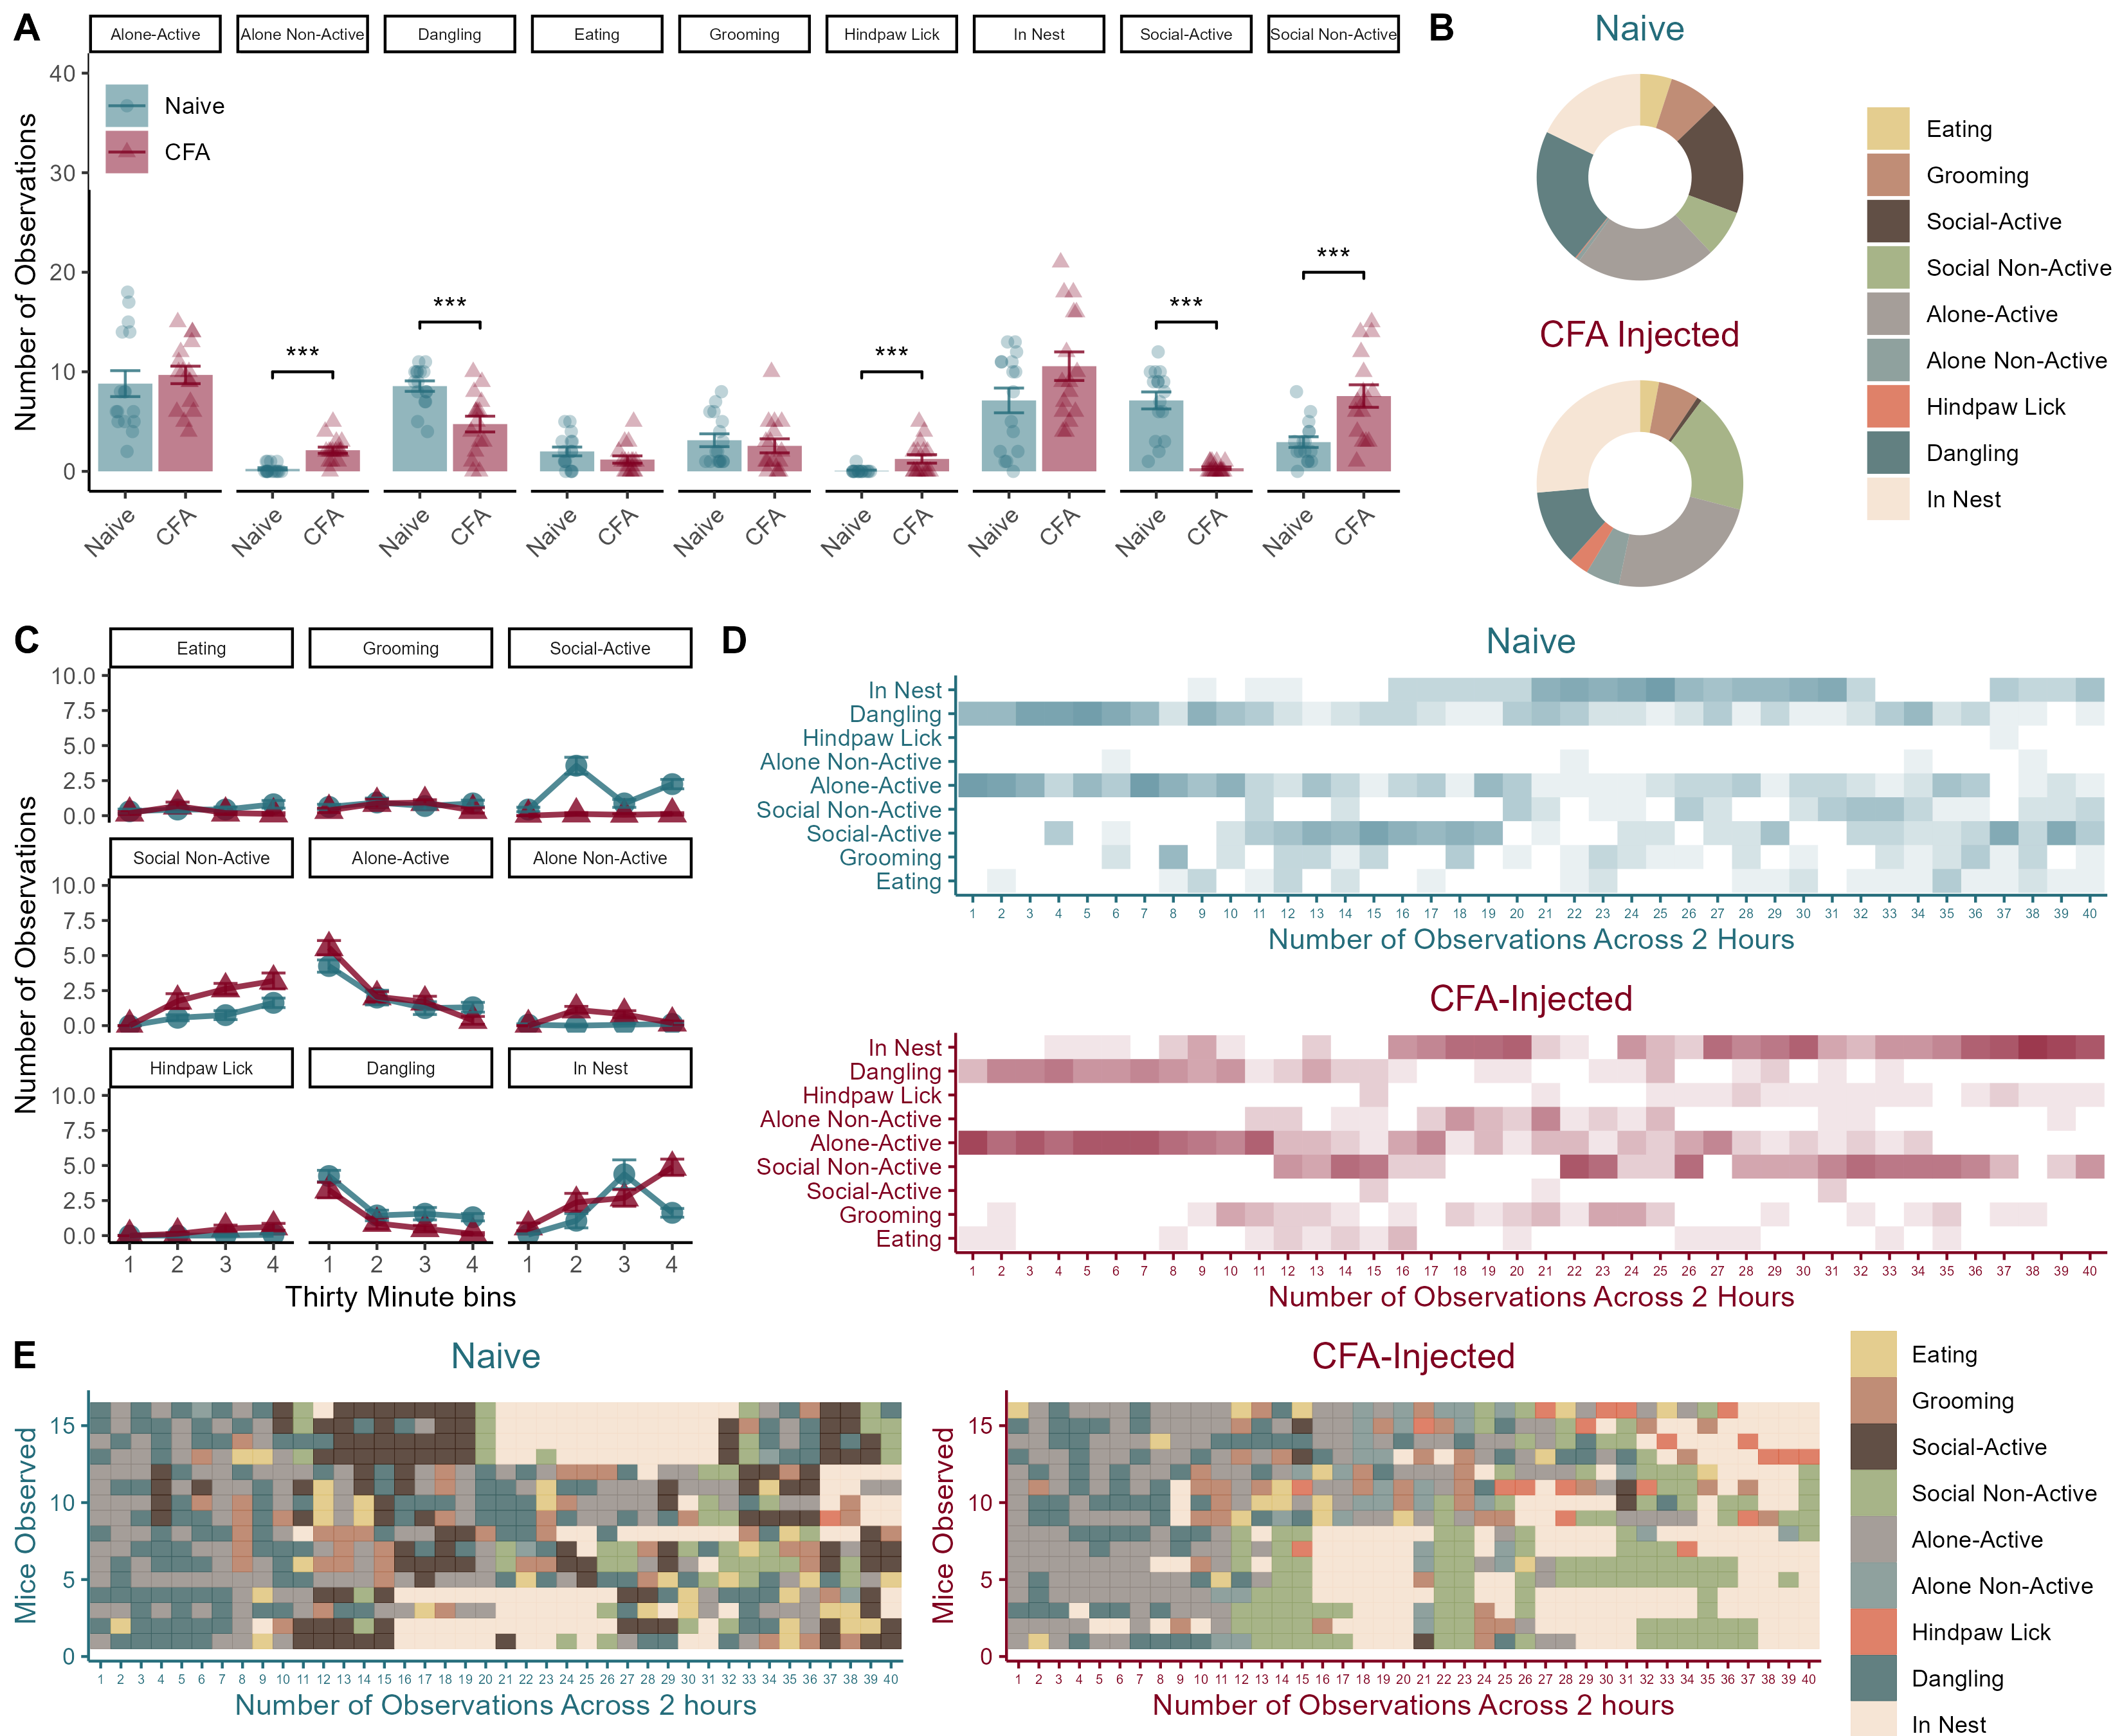
\includegraphics[width=45.83in]{Figs/1_male_HC_panel}

\textbf{Figure 1.} \emph{Homecage behaviors in male mice after an injection of 10}\(\mu l\) \emph{of 50\% CFA.} (A) Total number of observations of each behavior category across the two-hour observation period. (B) Donut charts showing the breakdown of average time spent engaging in each behavior for each group. (C) Line charts showcase group differences in changes in behavior across the two-hour long session. (D and E) are qualitative representations of the distribution of behaviors observed across the 40 time points. Data represented as mean value +/- SEM. \(***\) indicates p \textless{} 0.001.

\hypertarget{statistical-analyses}{%
\section*{Statistical Analyses}\label{statistical-analyses}}
\addcontentsline{toc}{section}{Statistical Analyses}

\hypertarget{overall-manova-for-hc-behavs-for-males}{%
\subsection*{Overall MANOVA for HC Behavs for males}\label{overall-manova-for-hc-behavs-for-males}}
\addcontentsline{toc}{subsection}{Overall MANOVA for HC Behavs for males}

\begin{Shaded}
\begin{Highlighting}[]
\CommentTok{\# All behaviours in the model throws an error {-} it knows that you need to leave one out I suppose. }

\CommentTok{\# It is important to leave one behavior out of the MANOVA to allow for a degree of freedom in the analysis. }

\DocumentationTok{\#\# I thought originally that I would leave time in the nest out, but bc there is a clear sex difference in that behaviour I chose eating instead here: }

\NormalTok{fit }\OtherTok{\textless{}{-}} \FunctionTok{manova}\NormalTok{(}\FunctionTok{cbind}\NormalTok{(Grooming,}\StringTok{\textasciigrave{}}\AttributeTok{Social{-}Active}\StringTok{\textasciigrave{}}\NormalTok{,}\StringTok{\textasciigrave{}}\AttributeTok{Social Non{-}Active}\StringTok{\textasciigrave{}}\NormalTok{,}\StringTok{\textasciigrave{}}\AttributeTok{Alone{-}Active}\StringTok{\textasciigrave{}}\NormalTok{,}\StringTok{\textasciigrave{}}\AttributeTok{Alone Non{-}Active}\StringTok{\textasciigrave{}}\NormalTok{,}\StringTok{\textasciigrave{}}\AttributeTok{Hindpaw Lick}\StringTok{\textasciigrave{}}\NormalTok{,}\StringTok{\textasciigrave{}}\AttributeTok{Dangling}\StringTok{\textasciigrave{}}\NormalTok{,}\StringTok{\textasciigrave{}}\AttributeTok{In Nest}\StringTok{\textasciigrave{}}\NormalTok{) }\SpecialCharTok{\textasciitilde{}}\NormalTok{ Condition, }\AttributeTok{data=}\NormalTok{b)}
\FunctionTok{summary}\NormalTok{(fit)}
\end{Highlighting}
\end{Shaded}

\begin{verbatim}
##            Df Pillai approx F num Df den Df                Pr(>F)    
## Condition   1  0.536   17.183      8    119 < 0.00000000000000022 ***
## Residuals 126                                                        
## ---
## Signif. codes:  0 '***' 0.001 '**' 0.01 '*' 0.05 '.' 0.1 ' ' 1
\end{verbatim}

\begin{itemize}
\tightlist
\item
  The overall MANOVA for males was significant (F(1,30) = 43.46, p \textless{} 0.001), indicating that 10 \(\mu l\) of 50\% CFA altered patterns of behaviour during the two-hour interval after injection.
\end{itemize}

\hypertarget{follow-up-analyses}{%
\subsection*{Follow up analyses}\label{follow-up-analyses}}
\addcontentsline{toc}{subsection}{Follow up analyses}

\begin{Shaded}
\begin{Highlighting}[]
\CommentTok{\# Prints out the individual ANOVAs for each behaviour}
\FunctionTok{summary.aov}\NormalTok{(fit)}
\end{Highlighting}
\end{Shaded}

\begin{verbatim}
##  Response Grooming :
##              Df  Sum Sq Mean Sq F value Pr(>F)
## Condition     1   0.633 0.63281  0.7691 0.3822
## Residuals   126 103.672 0.82279               
## 
##  Response Social-Active :
##              Df Sum Sq Mean Sq F value           Pr(>F)    
## Condition     1  92.82  92.820   50.51 0.00000000007788 ***
## Residuals   126 231.55   1.838                             
## ---
## Signif. codes:  0 '***' 0.001 '**' 0.01 '*' 0.05 '.' 0.1 ' ' 1
## 
##  Response Social Non-Active :
##              Df Sum Sq Mean Sq F value    Pr(>F)    
## Condition     1  42.78  42.781  15.729 0.0001219 ***
## Residuals   126 342.72   2.720                      
## ---
## Signif. codes:  0 '***' 0.001 '**' 0.01 '*' 0.05 '.' 0.1 ' ' 1
## 
##  Response Alone-Active :
##              Df Sum Sq Mean Sq F value Pr(>F)
## Condition     1   1.53  1.5313  0.2959 0.5874
## Residuals   126 651.97  5.1744               
## 
##  Response Alone Non-Active :
##              Df Sum Sq Mean Sq F value     Pr(>F)    
## Condition     1  7.031  7.0312   17.83 0.00004588 ***
## Residuals   126 49.688  0.3943                       
## ---
## Signif. codes:  0 '***' 0.001 '**' 0.01 '*' 0.05 '.' 0.1 ' ' 1
## 
##  Response Hindpaw Lick :
##              Df Sum Sq Mean Sq F value   Pr(>F)   
## Condition     1  2.820 2.82031  10.231 0.001747 **
## Residuals   126 34.734 0.27567                    
## ---
## Signif. codes:  0 '***' 0.001 '**' 0.01 '*' 0.05 '.' 0.1 ' ' 1
## 
##  Response Dangling :
##              Df Sum Sq Mean Sq F value  Pr(>F)   
## Condition     1  29.07 29.0703  8.3725 0.00449 **
## Residuals   126 437.48  3.4721                   
## ---
## Signif. codes:  0 '***' 0.001 '**' 0.01 '*' 0.05 '.' 0.1 ' ' 1
## 
##  Response In Nest :
##              Df Sum Sq Mean Sq F value  Pr(>F)  
## Condition     1  23.63 23.6328   3.332 0.07031 .
## Residuals   126 893.67  7.0926                  
## ---
## Signif. codes:  0 '***' 0.001 '**' 0.01 '*' 0.05 '.' 0.1 ' ' 1
\end{verbatim}

\begin{itemize}
\tightlist
\item
  Male mice that were injected with CFA exhibited fewer socially-active behaviours (F(1,30) = 66.62, p \textless{} 0.001),
\item
  More socially inactive behaviours (F(1,30) = 14.55, p \textless{} 0.001),
\item
  More hindpaw licks (F(1,30) = 8.07, p = 0.008),
\item
  And less time dangling (F(1,30) = 17.19, p \textless{} 0.001).
\end{itemize}

\emph{Note} that the non-statistically significant results shown above are not reported in the mauscript.

\hypertarget{figure-2---female-mice-homecage-behaviors-after-cfa}{%
\chapter*{Figure 2 - Female Mice: Homecage Behaviors after CFA}\label{figure-2---female-mice-homecage-behaviors-after-cfa}}
\addcontentsline{toc}{chapter}{Figure 2 - Female Mice: Homecage Behaviors after CFA}

\hypertarget{published-image-1}{%
\section*{Published Image}\label{published-image-1}}
\addcontentsline{toc}{section}{Published Image}

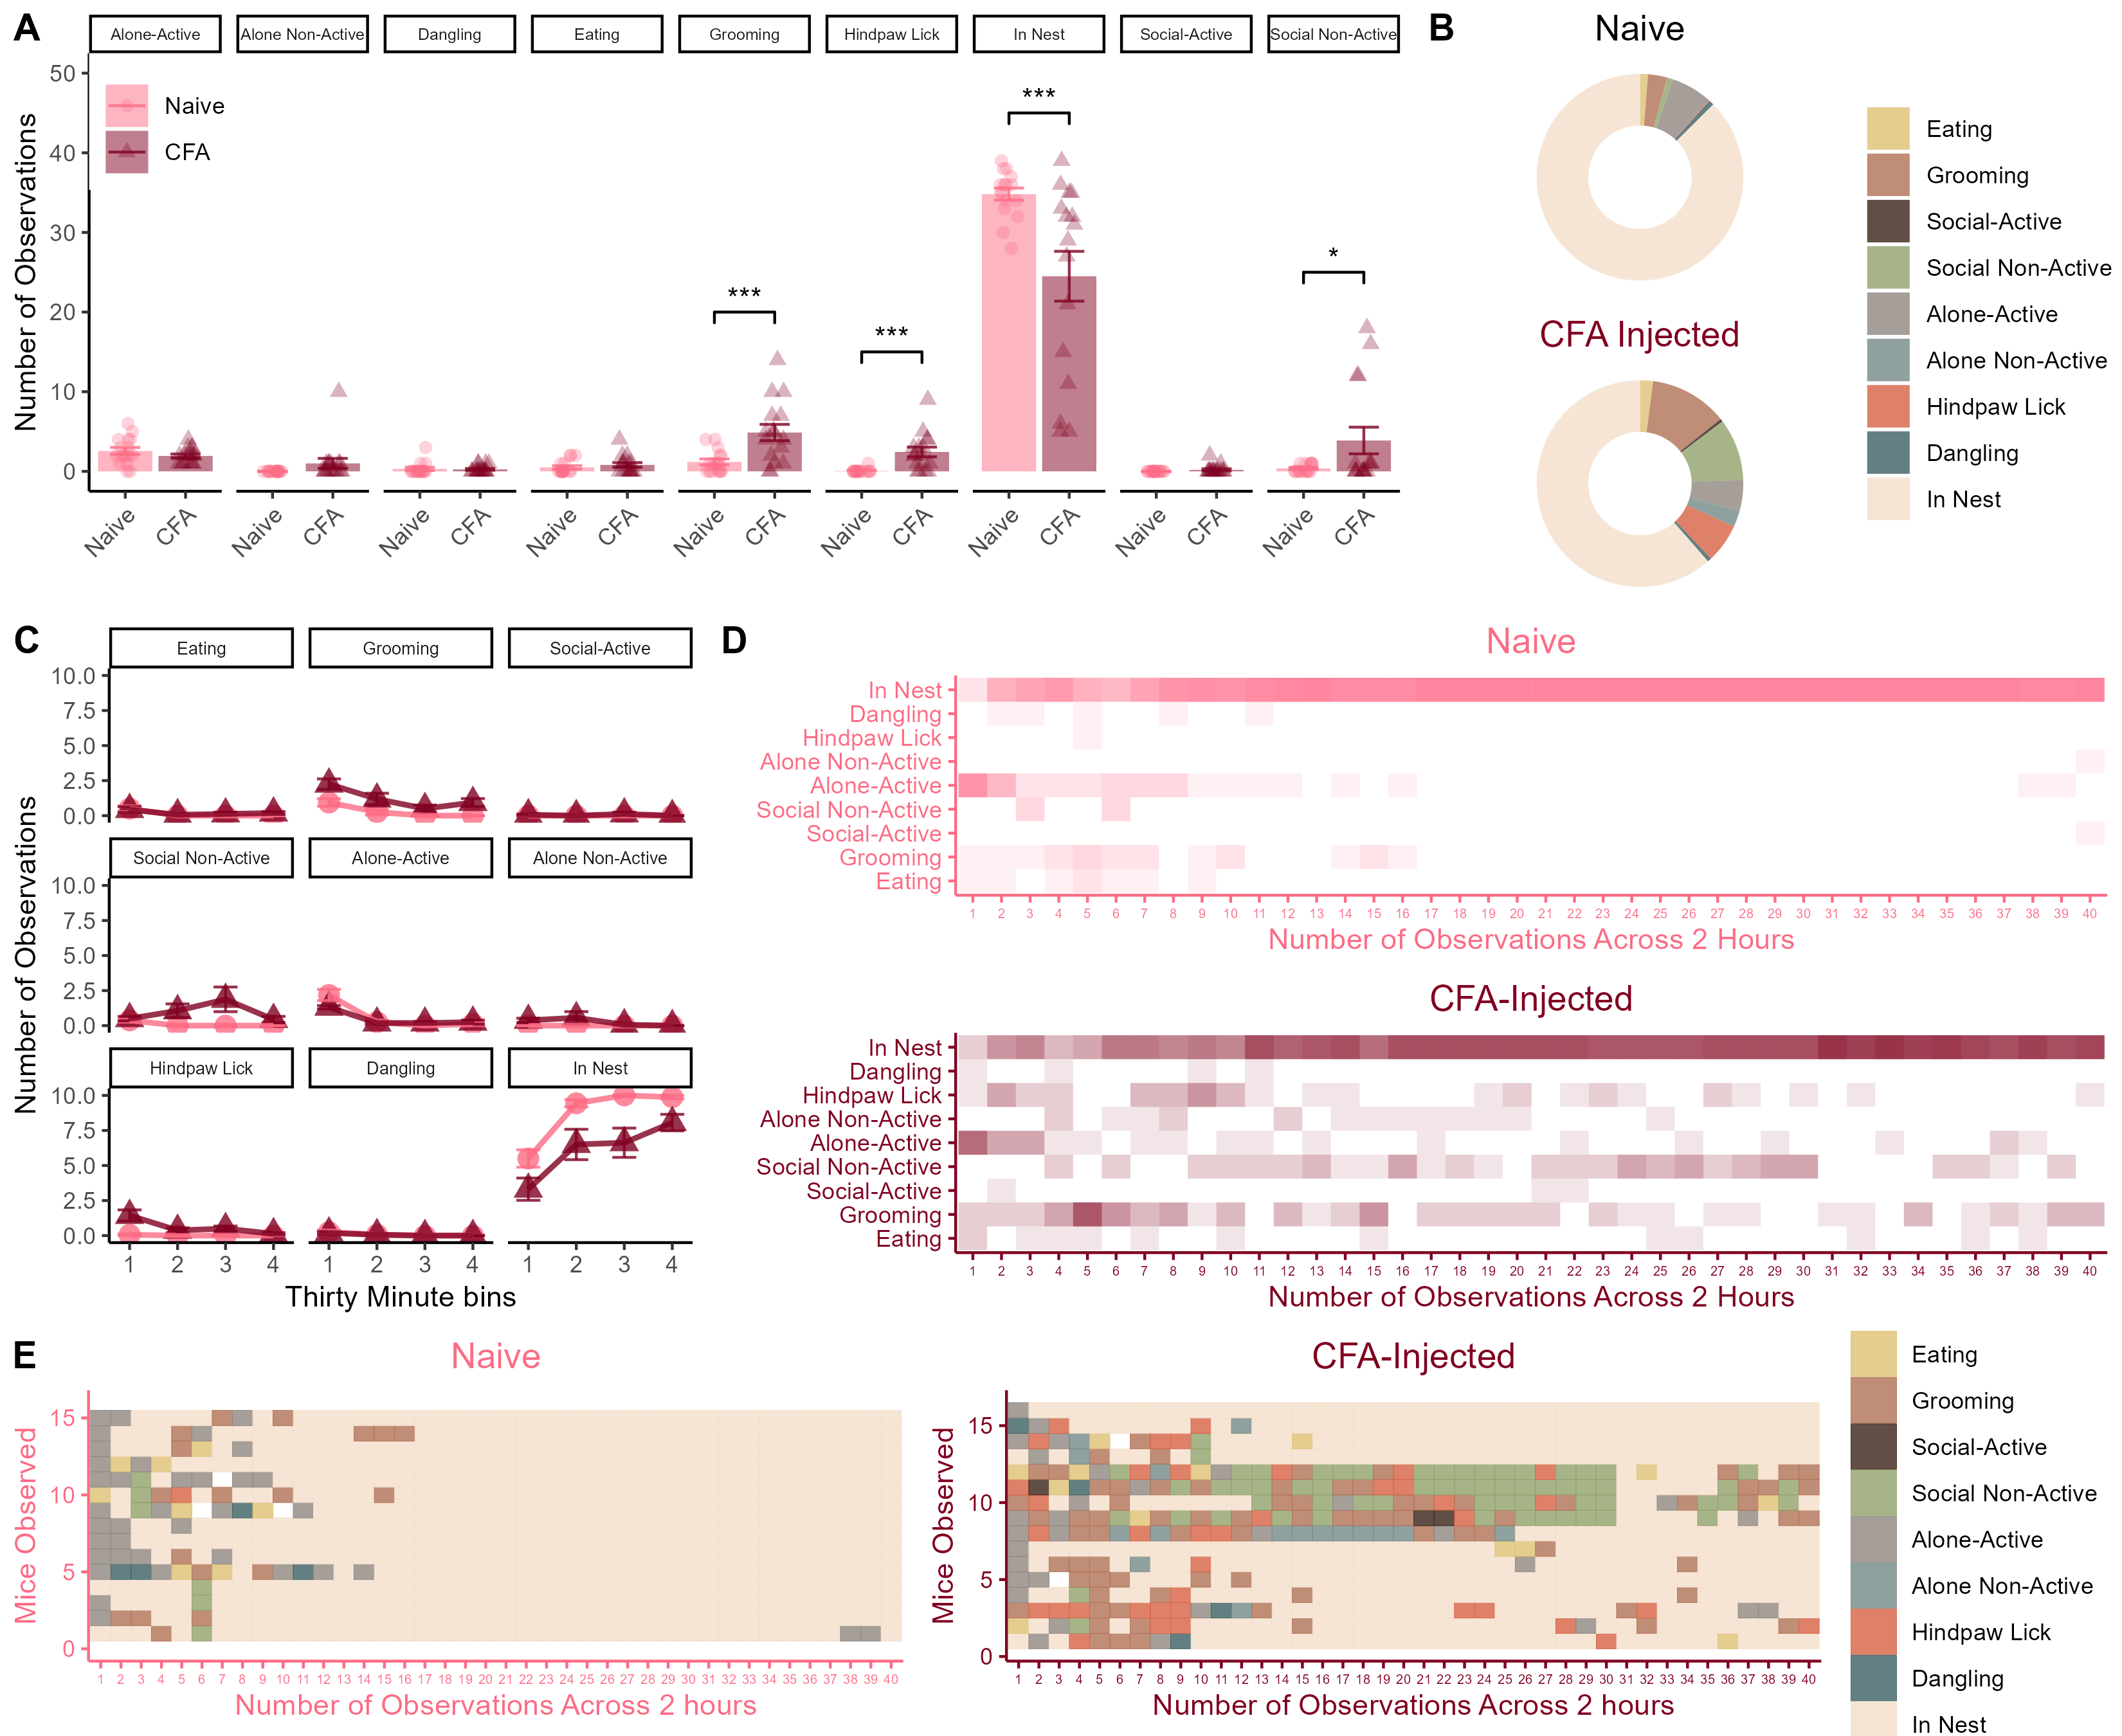
\includegraphics[width=45.83in]{Figs/2_female_HC_panel}

\textbf{Figure 2.} \emph{Homecage behaviors in female mice after injection of 10}\(\mu l\) \emph{of 50\% CFA.} (A) Total number of observations of each behavior category across the two-hour observation period. (B) Donut charts showing the breakdown of average time spent engaging in each behavior for each group. (C) Line charts showcase group differences in changes in behavior across the two-hour long session. (D and E) are qualitative representations of the distribution of behaviors observed across the 40 time points. Data represented as mean value +/- SEM. \(***\) indicates p \textless{} 0.001.

\hypertarget{statistical-analyses-1}{%
\section*{Statistical Analyses}\label{statistical-analyses-1}}
\addcontentsline{toc}{section}{Statistical Analyses}

\hypertarget{overall-manova-for-hc-behavs-for-females}{%
\subsection{Overall MANOVA for HC Behavs for females}\label{overall-manova-for-hc-behavs-for-females}}

\begin{Shaded}
\begin{Highlighting}[]
\CommentTok{\# All behaviours in the model throws an error {-} it knows that you need to leave one out I suppose. }
\DocumentationTok{\#\# I thought originally that I would leave time in the nest out, but bc there is a clear sex difference in that behaviour I chose eating instead here: }

\NormalTok{fit }\OtherTok{\textless{}{-}} \FunctionTok{manova}\NormalTok{(}\FunctionTok{cbind}\NormalTok{(Grooming,}\StringTok{\textasciigrave{}}\AttributeTok{Social{-}Active}\StringTok{\textasciigrave{}}\NormalTok{,}\StringTok{\textasciigrave{}}\AttributeTok{Social Non{-}Active}\StringTok{\textasciigrave{}}\NormalTok{,}\StringTok{\textasciigrave{}}\AttributeTok{Alone{-}Active}\StringTok{\textasciigrave{}}\NormalTok{,}\StringTok{\textasciigrave{}}\AttributeTok{Alone Non{-}Active}\StringTok{\textasciigrave{}}\NormalTok{,}\StringTok{\textasciigrave{}}\AttributeTok{Hindpaw Lick}\StringTok{\textasciigrave{}}\NormalTok{,}\StringTok{\textasciigrave{}}\AttributeTok{Dangling}\StringTok{\textasciigrave{}}\NormalTok{,}\StringTok{\textasciigrave{}}\AttributeTok{In Nest}\StringTok{\textasciigrave{}}\NormalTok{) }\SpecialCharTok{\textasciitilde{}}\NormalTok{ Condition, }\AttributeTok{data=}\NormalTok{b)}
\FunctionTok{summary}\NormalTok{(fit)}
\end{Highlighting}
\end{Shaded}

\begin{verbatim}
##            Df Pillai approx F num Df den Df      Pr(>F)    
## Condition   1 0.2647    5.355      8    119 0.000009378 ***
## Residuals 126                                              
## ---
## Signif. codes:  0 '***' 0.001 '**' 0.01 '*' 0.05 '.' 0.1 ' ' 1
\end{verbatim}

\begin{itemize}
\tightlist
\item
  The overall MANOVA for female mice was also significant (F(1,30) = 3.05, p = 0.017)
\end{itemize}

\hypertarget{follow-up}{%
\subsection{Follow up:}\label{follow-up}}

\begin{Shaded}
\begin{Highlighting}[]
\CommentTok{\# Prints out the individual ANOVAs for each behaviour}
\FunctionTok{summary.aov}\NormalTok{(fit)}
\end{Highlighting}
\end{Shaded}

\begin{verbatim}
##  Response Grooming :
##              Df  Sum Sq Mean Sq F value     Pr(>F)    
## Condition     1  27.195 27.1953  20.121 0.00001617 ***
## Residuals   126 170.297  1.3516                       
## ---
## Signif. codes:  0 '***' 0.001 '**' 0.01 '*' 0.05 '.' 0.1 ' ' 1
## 
##  Response Social-Active :
##              Df Sum Sq  Mean Sq F value Pr(>F)
## Condition     1 0.0703 0.070313  1.8232 0.1794
## Residuals   126 4.8594 0.038566               
## 
##  Response Social Non-Active :
##              Df Sum Sq Mean Sq F value   Pr(>F)   
## Condition     1  24.50 24.5000  10.742 0.001354 **
## Residuals   126 287.38  2.2808                    
## ---
## Signif. codes:  0 '***' 0.001 '**' 0.01 '*' 0.05 '.' 0.1 ' ' 1
## 
##  Response Alone-Active :
##              Df  Sum Sq Mean Sq F value Pr(>F)
## Condition     1   0.781 0.78125  0.7768 0.3798
## Residuals   126 126.719 1.00570               
## 
##  Response Alone Non-Active :
##              Df Sum Sq Mean Sq F value  Pr(>F)  
## Condition     1      2 2.00000     4.5 0.03585 *
## Residuals   126     56 0.44444                  
## ---
## Signif. codes:  0 '***' 0.001 '**' 0.01 '*' 0.05 '.' 0.1 ' ' 1
## 
##  Response Hindpaw Lick :
##              Df Sum Sq Mean Sq F value     Pr(>F)    
## Condition     1 11.281 11.2813  19.682 0.00001971 ***
## Residuals   126 72.219  0.5732                       
## ---
## Signif. codes:  0 '***' 0.001 '**' 0.01 '*' 0.05 '.' 0.1 ' ' 1
## 
##  Response Dangling :
##              Df  Sum Sq  Mean Sq F value Pr(>F)
## Condition     1  0.0078 0.007813   0.095 0.7584
## Residuals   126 10.3594 0.082217               
## 
##  Response In Nest :
##              Df Sum Sq Mean Sq F value     Pr(>F)    
## Condition     1  212.7 212.695  20.546 0.00001336 ***
## Residuals   126 1304.4  10.352                       
## ---
## Signif. codes:  0 '***' 0.001 '**' 0.01 '*' 0.05 '.' 0.1 ' ' 1
\end{verbatim}

CFA-injected Female mice exhibited:

\begin{itemize}
\tightlist
\item
  Increased grooming during the observation session (F(1,30) = 12.26, p = 0.0015)
\item
  Increased social inactive behaviour (F(1,30) = 4.626, p = 0.039)
\item
  More hindpaw licks (F(1,30) = 15.95, p \textless{} 0.001)
\item
  And less observations in the nest (F(1,30) = 10.93, p = 0.002)
\end{itemize}

\begin{Shaded}
\begin{Highlighting}[]
\NormalTok{knitr}\SpecialCharTok{::}\NormalTok{opts\_chunk}\SpecialCharTok{$}\FunctionTok{set}\NormalTok{(}\AttributeTok{message =} \ConstantTok{FALSE}\NormalTok{, }
                      \AttributeTok{warning =} \ConstantTok{FALSE}\NormalTok{,}
                      \AttributeTok{echo =} \ConstantTok{FALSE}\NormalTok{,}
                      \AttributeTok{fig.align =} \StringTok{\textquotesingle{}center\textquotesingle{}}\NormalTok{)}
\FunctionTok{options}\NormalTok{(}\AttributeTok{scipen =} \DecValTok{999}\NormalTok{)}
\end{Highlighting}
\end{Shaded}

\hypertarget{figure-3---recovery-from-cfa-injury}{%
\chapter*{Figure 3 - Recovery from CFA Injury}\label{figure-3---recovery-from-cfa-injury}}
\addcontentsline{toc}{chapter}{Figure 3 - Recovery from CFA Injury}

\hypertarget{published-image-2}{%
\section*{Published Image}\label{published-image-2}}
\addcontentsline{toc}{section}{Published Image}

\begin{center}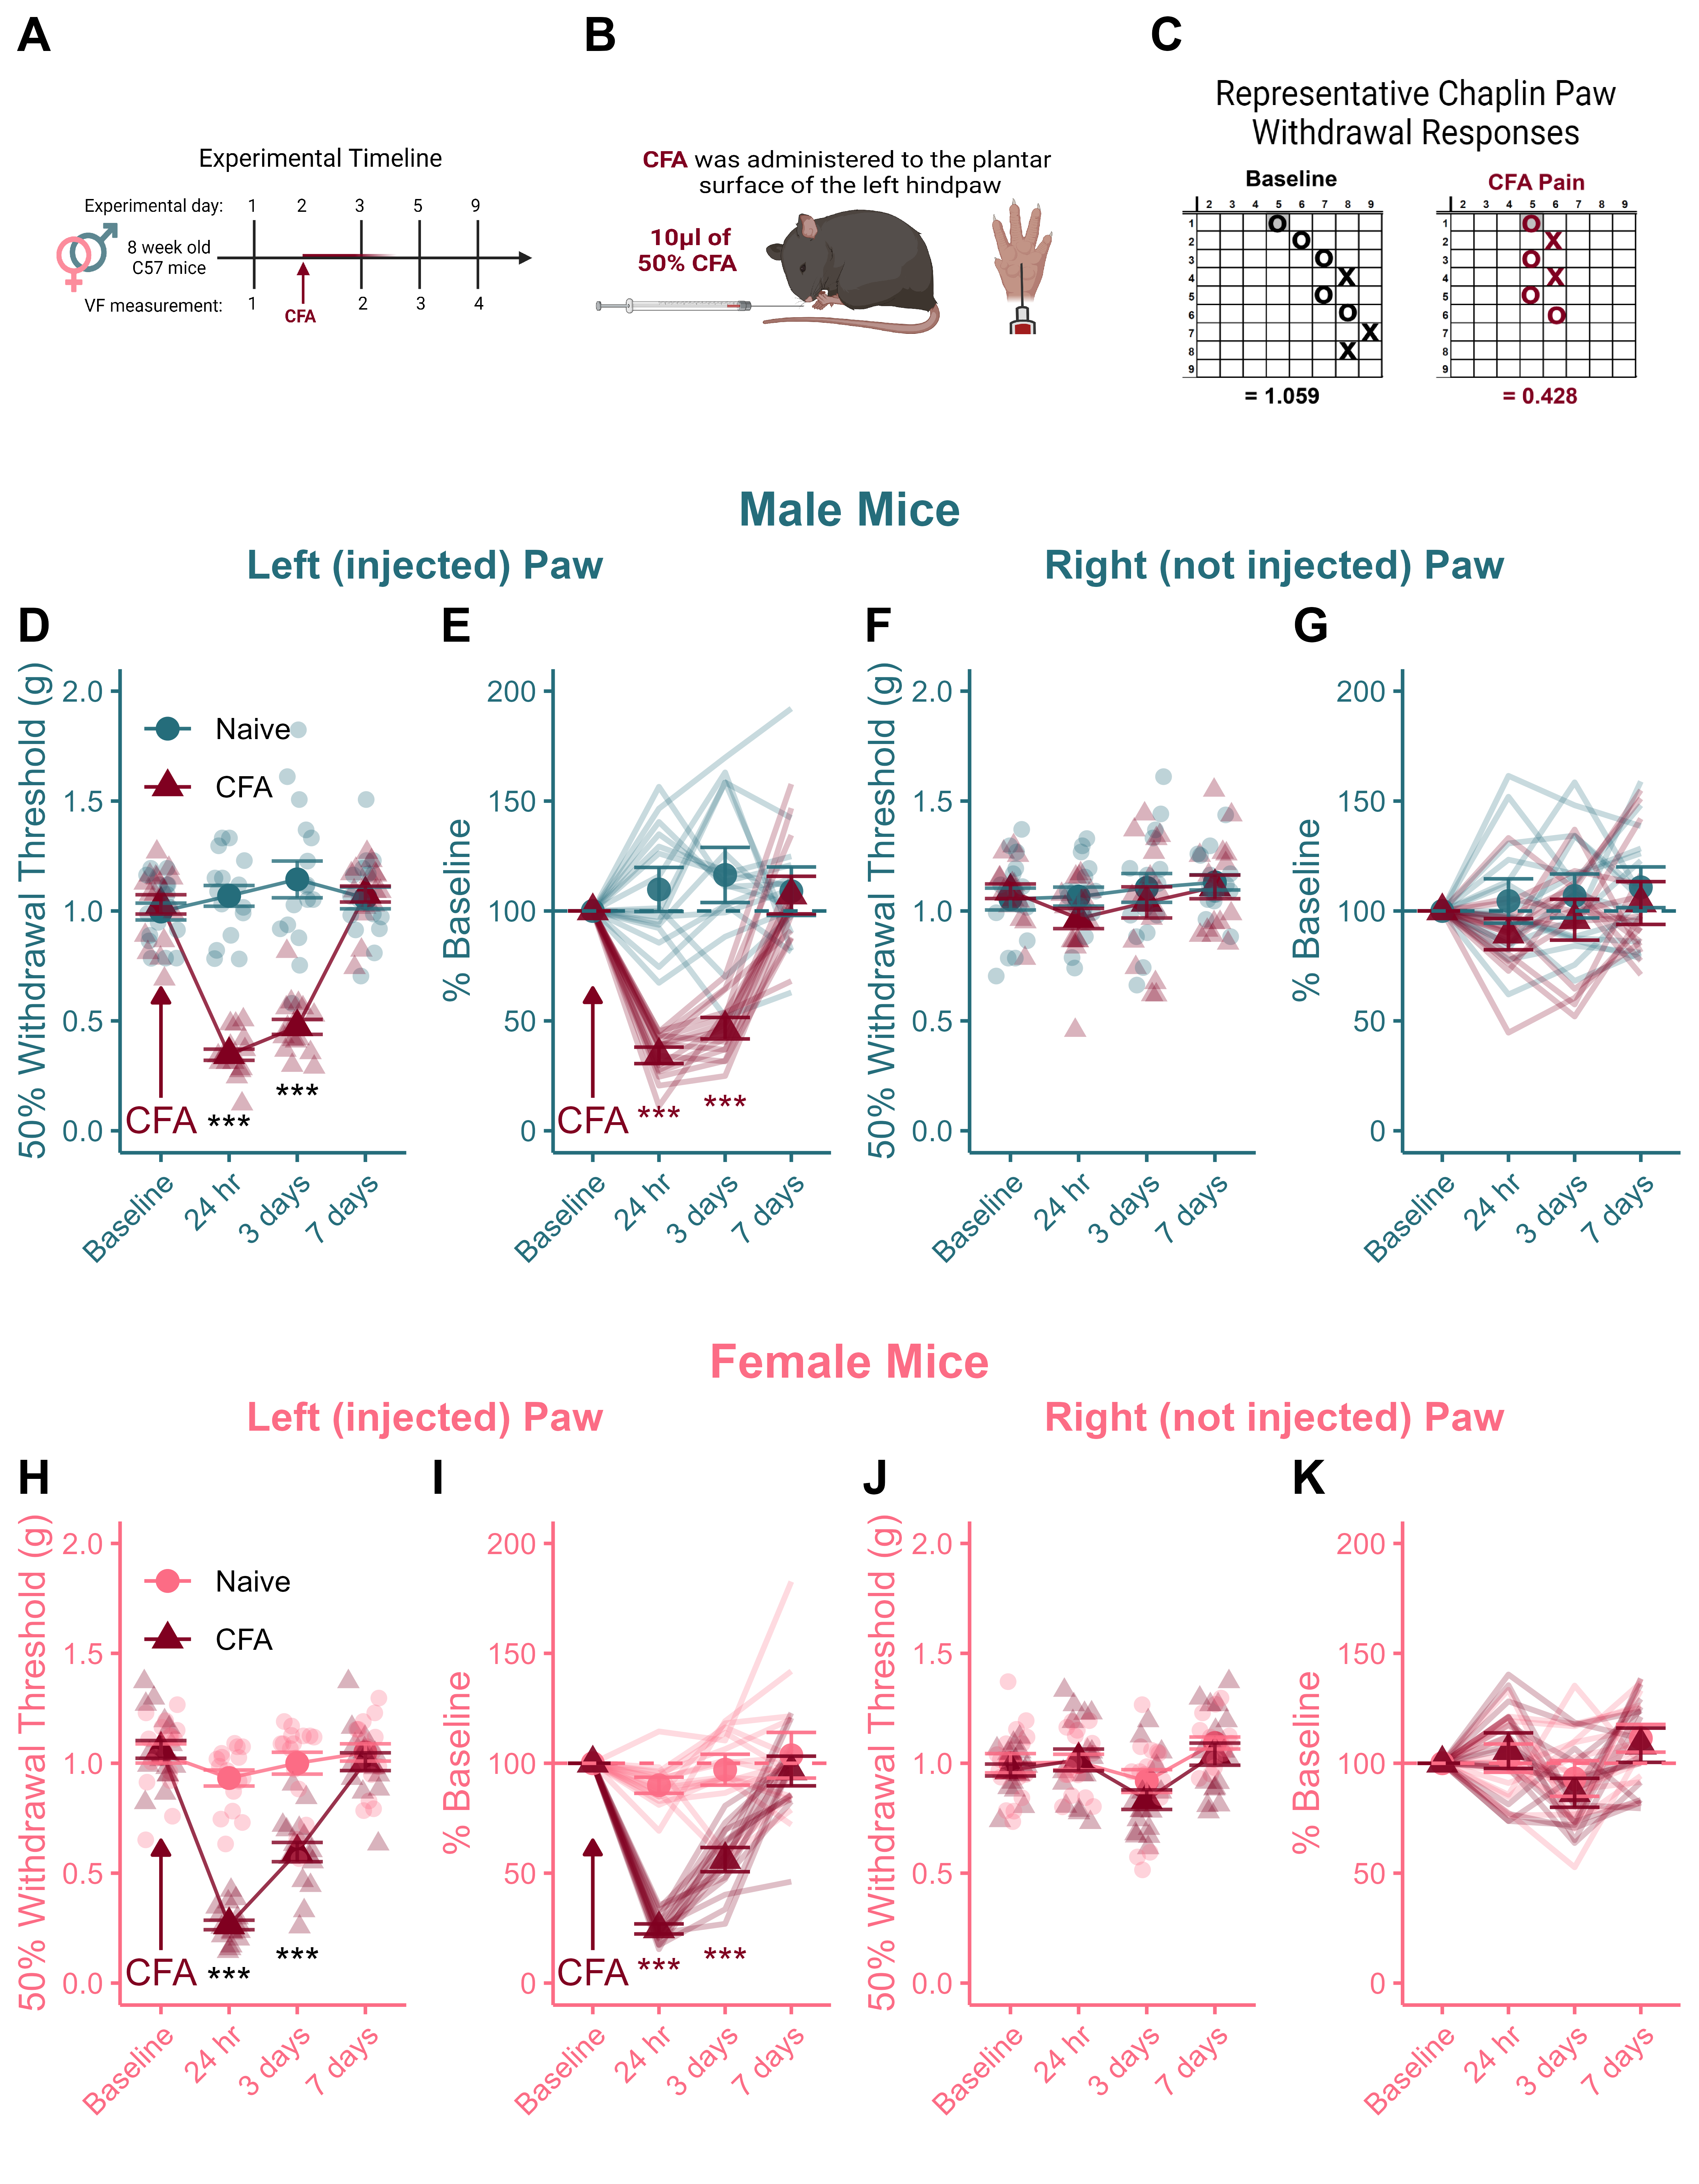
\includegraphics[width=68.06in]{Figs/3_VF_CFA_Recovery} \end{center}

\textbf{Figure 3.} \emph{CFA injection produces mechanical hypersensitivity that resolves within 7 days in male and female mice.} (A) Timeline of experimental testing. (B) Pain model to induce sensitization. (C) Representative images of Chaplan up-down von Frey measurements after CFA injection. CFA administration produces robust hypersensitivity at the site of injection that persists for at least 3 days and resolves within one week in both male (D, E) and female (H, I) mice. There were no changes in sensitivity of the contralateral (non-injected; right) hind paw during inflammatory pain and recovery from CFA injury in either males (F, G) or females (J, K). Data expressed as mean +/- SEM. \(***\) Indicates between-group difference where \emph{p} \textless{} 0.001 and \# indicates a within-subject difference from baseline where \emph{p} \textless{} 0.05.

\hypertarget{statistical-analyses-2}{%
\section*{Statistical Analyses}\label{statistical-analyses-2}}
\addcontentsline{toc}{section}{Statistical Analyses}

\begin{Shaded}
\begin{Highlighting}[]
\CommentTok{\# Select the left paws}
\NormalTok{left\_paws }\OtherTok{\textless{}{-}} \FunctionTok{rbind}\NormalTok{(female\_left,male\_left)}

\CommentTok{\# Switch to long form}
\NormalTok{a }\OtherTok{\textless{}{-}}\NormalTok{ left\_paws }\SpecialCharTok{\%\textgreater{}\%} 
  \FunctionTok{melt}\NormalTok{(}\AttributeTok{id.vars=}\FunctionTok{c}\NormalTok{(}\StringTok{"ID"}\NormalTok{,}\StringTok{"Sex"}\NormalTok{,}\StringTok{"CFA"}\NormalTok{))}

\CommentTok{\# Run RM anova on the 4 days of VF measuremenets}
\NormalTok{b }\OtherTok{\textless{}{-}} \FunctionTok{anova\_test}\NormalTok{(}\AttributeTok{data=}\NormalTok{a, }\AttributeTok{dv=}\NormalTok{value,}\AttributeTok{wid=}\NormalTok{ID,}\AttributeTok{between=}\FunctionTok{c}\NormalTok{(CFA,Sex),}\AttributeTok{within=}\NormalTok{variable,}\AttributeTok{effect.size=}\StringTok{"pes"}\NormalTok{)}
\NormalTok{knitr}\SpecialCharTok{::}\FunctionTok{kable}\NormalTok{(}\FunctionTok{get\_anova\_table}\NormalTok{(b))}
\end{Highlighting}
\end{Shaded}

\begin{tabular}{l|r|r|r|r|l|r}
\hline
Effect & DFn & DFd & F & p & p<.05 & pes\\
\hline
CFA & 1 & 60 & 128.271 & 0.000 & * & 0.681\\
\hline
Sex & 1 & 60 & 1.211 & 0.275 &  & 0.020\\
\hline
variable & 3 & 180 & 99.726 & 0.000 & * & 0.624\\
\hline
CFA:Sex & 1 & 60 & 1.314 & 0.256 &  & 0.021\\
\hline
CFA:variable & 3 & 180 & 91.678 & 0.000 & * & 0.604\\
\hline
Sex:variable & 3 & 180 & 2.651 & 0.050 &  & 0.042\\
\hline
CFA:Sex:variable & 3 & 180 & 3.570 & 0.015 & * & 0.056\\
\hline
\end{tabular}

\begin{itemize}
\item
  Significant main effects of CFA and timepoint.
\item
  Significant interaction between CFA and timepoint (F(3,180) = 91.67, p \textless{} 0.001)
\item
  Significant 3-way interaction between Sex, CFA and timepoint (F(3,180) = 3.57, p = 0.015)
\end{itemize}

\begin{Shaded}
\begin{Highlighting}[]
\CommentTok{\# Run two way ANOVAs for males and females separately: }

\DocumentationTok{\#\# Males}
\NormalTok{res }\OtherTok{\textless{}{-}}\NormalTok{ a }\SpecialCharTok{\%\textgreater{}\%}
  \FunctionTok{filter}\NormalTok{(Sex }\SpecialCharTok{==} \StringTok{"Male"}\NormalTok{) }\SpecialCharTok{\%\textgreater{}\%}
  \FunctionTok{anova\_test}\NormalTok{(}\AttributeTok{dv=}\NormalTok{value,}\AttributeTok{wid=}\NormalTok{ID,}\AttributeTok{between=}\NormalTok{CFA,}\AttributeTok{within=}\NormalTok{variable,}\AttributeTok{effect.size =} \StringTok{"pes"}\NormalTok{)}
\end{Highlighting}
\end{Shaded}

There is a significant interaction between CFA treatment and time point (F(3,90) = 47.44, p \textless{} 0.001)

\begin{Shaded}
\begin{Highlighting}[]
\DocumentationTok{\#\#\# Follow up for males: }
\NormalTok{res }\OtherTok{\textless{}{-}}\NormalTok{ a }\SpecialCharTok{\%\textgreater{}\%} 
  \FunctionTok{filter}\NormalTok{(Sex }\SpecialCharTok{==} \StringTok{"Male"}\NormalTok{) }\SpecialCharTok{\%\textgreater{}\%}
  \FunctionTok{group\_by}\NormalTok{(variable) }\SpecialCharTok{\%\textgreater{}\%}
  \FunctionTok{pairwise\_t\_test}\NormalTok{(value}\SpecialCharTok{\textasciitilde{}}\NormalTok{CFA,}\AttributeTok{p.adjust.method =} \StringTok{"bonferroni"}\NormalTok{)}

\FunctionTok{tt}\NormalTok{(res)}
\end{Highlighting}
\end{Shaded}

\begin{table}
\centering
\begin{tblr}[         %% tabularray outer open
]                     %% tabularray outer close
{                     %% tabularray inner open
colspec={Q[]Q[]Q[]Q[]Q[]Q[]Q[]Q[]Q[]Q[]},
}                     %% tabularray inner close
\toprule
variable & .y. & group1 & group2 & n1 & n2 & p & p.signif & p.adj & p.adj.signif \\ \midrule %% TinyTableHeader
BL_L   & value & Naive & CFA & 16 & 16 & 0.5679999999999999 & ns   & 0.5679999999999999 & ns   \\
hr_24  & value & Naive & CFA & 16 & 16 & 0.0000000000000122 & **** & 0.0000000000000122 & **** \\
days_3 & value & Naive & CFA & 16 & 16 & 0.0000000146000000 & **** & 0.0000000146000000 & **** \\
days_7 & value & Naive & CFA & 16 & 16 & 0.7670000000000000 & ns   & 0.7670000000000000 & ns   \\
\bottomrule
\end{tblr}
\end{table}

\begin{itemize}
\item
  CFA-injected males have lower paw withdrawal thresholds than naive males 24 hours and 3 days post CFA administration (both p \textless{} 0.001).
\item
  There is no difference between the groups at baseline or 7 days post injection.
\end{itemize}

\begin{Shaded}
\begin{Highlighting}[]
\DocumentationTok{\#\# Females }
\NormalTok{a }\SpecialCharTok{\%\textgreater{}\%} 
  \FunctionTok{filter}\NormalTok{(Sex }\SpecialCharTok{==} \StringTok{"Female"}\NormalTok{) }\SpecialCharTok{\%\textgreater{}\%}
  \FunctionTok{anova\_test}\NormalTok{(}\AttributeTok{dv=}\NormalTok{value,}\AttributeTok{wid=}\NormalTok{ID,}\AttributeTok{between=}\NormalTok{CFA,}\AttributeTok{within=}\NormalTok{variable,}\AttributeTok{effect.size=}\StringTok{"pes"}\NormalTok{)}
\end{Highlighting}
\end{Shaded}

\begin{verbatim}
## ANOVA Table (type II tests)
## 
## $ANOVA
##         Effect DFn DFd      F                              p p<.05   pes
## 1          CFA   1  30 53.808 0.0000000359999999999999981061     * 0.642
## 2     variable   3  90 84.569 0.0000000000000000000000000427     * 0.738
## 3 CFA:variable   3  90 47.938 0.0000000000000000013200000000     * 0.615
## 
## $`Mauchly's Test for Sphericity`
##         Effect     W     p p<.05
## 1     variable 0.507 0.002     *
## 2 CFA:variable 0.507 0.002     *
## 
## $`Sphericity Corrections`
##         Effect   GGe      DF[GG]                    p[GG] p[GG]<.05   HFe
## 1     variable 0.754 2.26, 67.88 0.0000000000000000000289         * 0.819
## 2 CFA:variable 0.754 2.26, 67.88 0.0000000000000135000000         * 0.819
##       DF[HF]                      p[HF] p[HF]<.05
## 1 2.46, 73.7 0.000000000000000000000841         *
## 2 2.46, 73.7 0.000000000000001180000000         *
\end{verbatim}

\begin{itemize}
\tightlist
\item
  CFA-injected female mice also have lower paw withdrawal thresholds than naive males 24 hours and 3 days post CFA administration (both p \textless{} 0.001).
\end{itemize}

\begin{table}
\centering
\begin{tblr}[         %% tabularray outer open
]                     %% tabularray outer close
{                     %% tabularray inner open
colspec={Q[]Q[]Q[]Q[]Q[]Q[]Q[]Q[]Q[]Q[]},
}                     %% tabularray inner close
\toprule
variable & .y. & group1 & group2 & n1 & n2 & p & p.signif & p.adj & p.adj.signif \\ \midrule %% TinyTableHeader
BL_L   & value & Naive & CFA & 16 & 16 & 0.748999999999999999 & ns   & 0.748999999999999999 & ns   \\
hr_24  & value & Naive & CFA & 16 & 16 & 0.000000000000000195 & **** & 0.000000000000000195 & **** \\
days_3 & value & Naive & CFA & 16 & 16 & 0.000000594000000000 & **** & 0.000000594000000000 & **** \\
days_7 & value & Naive & CFA & 16 & 16 & 0.446000000000000008 & ns   & 0.446000000000000008 & ns   \\
\bottomrule
\end{tblr}
\end{table}

\begin{itemize}
\item
  CFA-injected males have lower paw withdrawal thresholds than naive males 24 hours and 3 days post CFA administration (both p \textless{} 0.001).
\item
  There is no difference between the groups at baseline or 7 days post injection.
\end{itemize}

\begin{Shaded}
\begin{Highlighting}[]
\CommentTok{\# Follow up the significant 3{-}way interaction using piarwise comparisons by invstigating the effect of Sex on each day of testing split by CFA}
\NormalTok{res }\OtherTok{\textless{}{-}}\NormalTok{ a }\SpecialCharTok{\%\textgreater{}\%}
  \FunctionTok{group\_by}\NormalTok{(CFA,variable) }\SpecialCharTok{\%\textgreater{}\%}
  \FunctionTok{pairwise\_t\_test}\NormalTok{(value}\SpecialCharTok{\textasciitilde{}}\NormalTok{Sex,}\AttributeTok{p.adjust.method =} \StringTok{"bonferroni"}\NormalTok{)}

\FunctionTok{tt}\NormalTok{(res)}
\end{Highlighting}
\end{Shaded}

\begin{table}
\centering
\begin{tblr}[         %% tabularray outer open
]                     %% tabularray outer close
{                     %% tabularray inner open
colspec={Q[]Q[]Q[]Q[]Q[]Q[]Q[]Q[]Q[]Q[]Q[]},
}                     %% tabularray inner close
\toprule
CFA & variable & .y. & group1 & group2 & n1 & n2 & p & p.signif & p.adj & p.adj.signif \\ \midrule %% TinyTableHeader
Naive & BL_L   & value & Female & Male & 16 & 16 & 0.4080 & ns & 0.4080 & ns \\
Naive & hr_24  & value & Female & Male & 16 & 16 & 0.0254 & *  & 0.0254 & *  \\
Naive & days_3 & value & Female & Male & 16 & 16 & 0.1390 & ns & 0.1390 & ns \\
Naive & days_7 & value & Female & Male & 16 & 16 & 0.8710 & ns & 0.8710 & ns \\
CFA   & BL_L   & value & Female & Male & 16 & 16 & 0.5710 & ns & 0.5710 & ns \\
CFA   & hr_24  & value & Female & Male & 16 & 16 & 0.0170 & *  & 0.0170 & *  \\
CFA   & days_3 & value & Female & Male & 16 & 16 & 0.0288 & *  & 0.0288 & *  \\
CFA   & days_7 & value & Female & Male & 16 & 16 & 0.1940 & ns & 0.1940 & ns \\
\bottomrule
\end{tblr}
\end{table}

\begin{itemize}
\item
  There was a sex difference in CFA-induced hypersensitivity both 24 hours (p = 0.017) and 3 days (p = 0.0288) post injection.
\item
  Female mice exhibited MORE sensitivity than males at the 24hour time point, and LESS sensitivity than males 3-days after CFA.
\end{itemize}

\begin{Shaded}
\begin{Highlighting}[]
\DocumentationTok{\#\# Effect of day within each of the 4 groups (i.e., the same thing as the \% BL stat..)}
\DocumentationTok{\#\#\# Only read \& interpret measurements relative to BASELINE}

\NormalTok{b }\OtherTok{\textless{}{-}}\NormalTok{ a }\SpecialCharTok{\%\textgreater{}\%} \FunctionTok{group\_by}\NormalTok{(CFA,Sex) }\SpecialCharTok{\%\textgreater{}\%} 
  \FunctionTok{pairwise\_t\_test}\NormalTok{(value}\SpecialCharTok{\textasciitilde{}}\NormalTok{variable,}\AttributeTok{p.adjust.method =} \StringTok{"bonferroni"}\NormalTok{)}
\FunctionTok{tt}\NormalTok{(b)}
\end{Highlighting}
\end{Shaded}

\begin{table}
\centering
\begin{tblr}[         %% tabularray outer open
]                     %% tabularray outer close
{                     %% tabularray inner open
colspec={Q[]Q[]Q[]Q[]Q[]Q[]Q[]Q[]Q[]Q[]Q[]},
}                     %% tabularray inner close
\toprule
Sex & CFA & .y. & group1 & group2 & n1 & n2 & p & p.signif & p.adj & p.adj.signif \\ \midrule %% TinyTableHeader
Female & Naive & value & BL_L   & hr_24  & 16 & 16 & 0.060299999999999999433786 & ns   & 0.361999999999999988453681 & ns   \\
Female & Naive & value & BL_L   & days_3 & 16 & 16 & 0.452000000000000012878587 & ns   & 1.000000000000000000000000 & ns   \\
Female & Naive & value & hr_24  & days_3 & 16 & 16 & 0.252000000000000001776357 & ns   & 1.000000000000000000000000 & ns   \\
Female & Naive & value & BL_L   & days_7 & 16 & 16 & 0.936000000000000054178884 & ns   & 1.000000000000000000000000 & ns   \\
Female & Naive & value & hr_24  & days_7 & 16 & 16 & 0.050599999999999999145128 & ns   & 0.303999999999999992450483 & ns   \\
Female & Naive & value & days_3 & days_7 & 16 & 16 & 0.405000000000000026645353 & ns   & 1.000000000000000000000000 & ns   \\
Male   & Naive & value & BL_L   & hr_24  & 16 & 16 & 0.365999999999999992006394 & ns   & 1.000000000000000000000000 & ns   \\
Male   & Naive & value & BL_L   & days_3 & 16 & 16 & 0.067000000000000003996803 & ns   & 0.402000000000000023980817 & ns   \\
Male   & Naive & value & hr_24  & days_3 & 16 & 16 & 0.343000000000000027089442 & ns   & 1.000000000000000000000000 & ns   \\
Male   & Naive & value & BL_L   & days_7 & 16 & 16 & 0.432999999999999996003197 & ns   & 1.000000000000000000000000 & ns   \\
Male   & Naive & value & hr_24  & days_7 & 16 & 16 & 0.904000000000000025757174 & ns   & 1.000000000000000000000000 & ns   \\
Male   & Naive & value & days_3 & days_7 & 16 & 16 & 0.285999999999999976463272 & ns   & 1.000000000000000000000000 & ns   \\
Female & CFA   & value & BL_L   & hr_24  & 16 & 16 & 0.000000000000000000000110 & **** & 0.000000000000000000000659 & **** \\
Female & CFA   & value & BL_L   & days_3 & 16 & 16 & 0.000000000000723000000000 & **** & 0.000000000004340000000000 & **** \\
Female & CFA   & value & hr_24  & days_3 & 16 & 16 & 0.000000021800000000000000 & **** & 0.000000130999999999999995 & **** \\
Female & CFA   & value & BL_L   & days_7 & 16 & 16 & 0.280000000000000026645353 & ns   & 1.000000000000000000000000 & ns   \\
Female & CFA   & value & hr_24  & days_7 & 16 & 16 & 0.000000000000000000003480 & **** & 0.000000000000000000020900 & **** \\
Female & CFA   & value & days_3 & days_7 & 16 & 16 & 0.000000000050700000000000 & **** & 0.000000000304000000000000 & **** \\
Male   & CFA   & value & BL_L   & hr_24  & 16 & 16 & 0.000000000000000000012500 & **** & 0.000000000000000000075000 & **** \\
Male   & CFA   & value & BL_L   & days_3 & 16 & 16 & 0.000000000000000101000000 & **** & 0.000000000000000606000000 & **** \\
Male   & CFA   & value & hr_24  & days_3 & 16 & 16 & 0.011700000000000000330291 & *    & 0.069900000000000003796963 & ns   \\
Male   & CFA   & value & BL_L   & days_7 & 16 & 16 & 0.338000000000000022648550 & ns   & 1.000000000000000000000000 & ns   \\
Male   & CFA   & value & hr_24  & days_7 & 16 & 16 & 0.000000000000000000000552 & **** & 0.000000000000000000003310 & **** \\
Male   & CFA   & value & days_3 & days_7 & 16 & 16 & 0.000000000000000003240000 & **** & 0.000000000000000019400000 & **** \\
\bottomrule
\end{tblr}
\end{table}

\begin{itemize}
\item
  CFA administration produced a robust hypersensitivity in the injected paw.
\item
  There was no evidence of sensitivity in the contralateral (non-injured) paw.
\item
  CFA-induced sensitivity resolved within one week post injection.
\end{itemize}

\hypertarget{figure-4---recovery-from-pge-2-injection}{%
\chapter*{Figure 4 - Recovery From PGE-2 Injection}\label{figure-4---recovery-from-pge-2-injection}}
\addcontentsline{toc}{chapter}{Figure 4 - Recovery From PGE-2 Injection}

\hypertarget{published-image-3}{%
\section*{Published Image}\label{published-image-3}}
\addcontentsline{toc}{section}{Published Image}

\begin{center}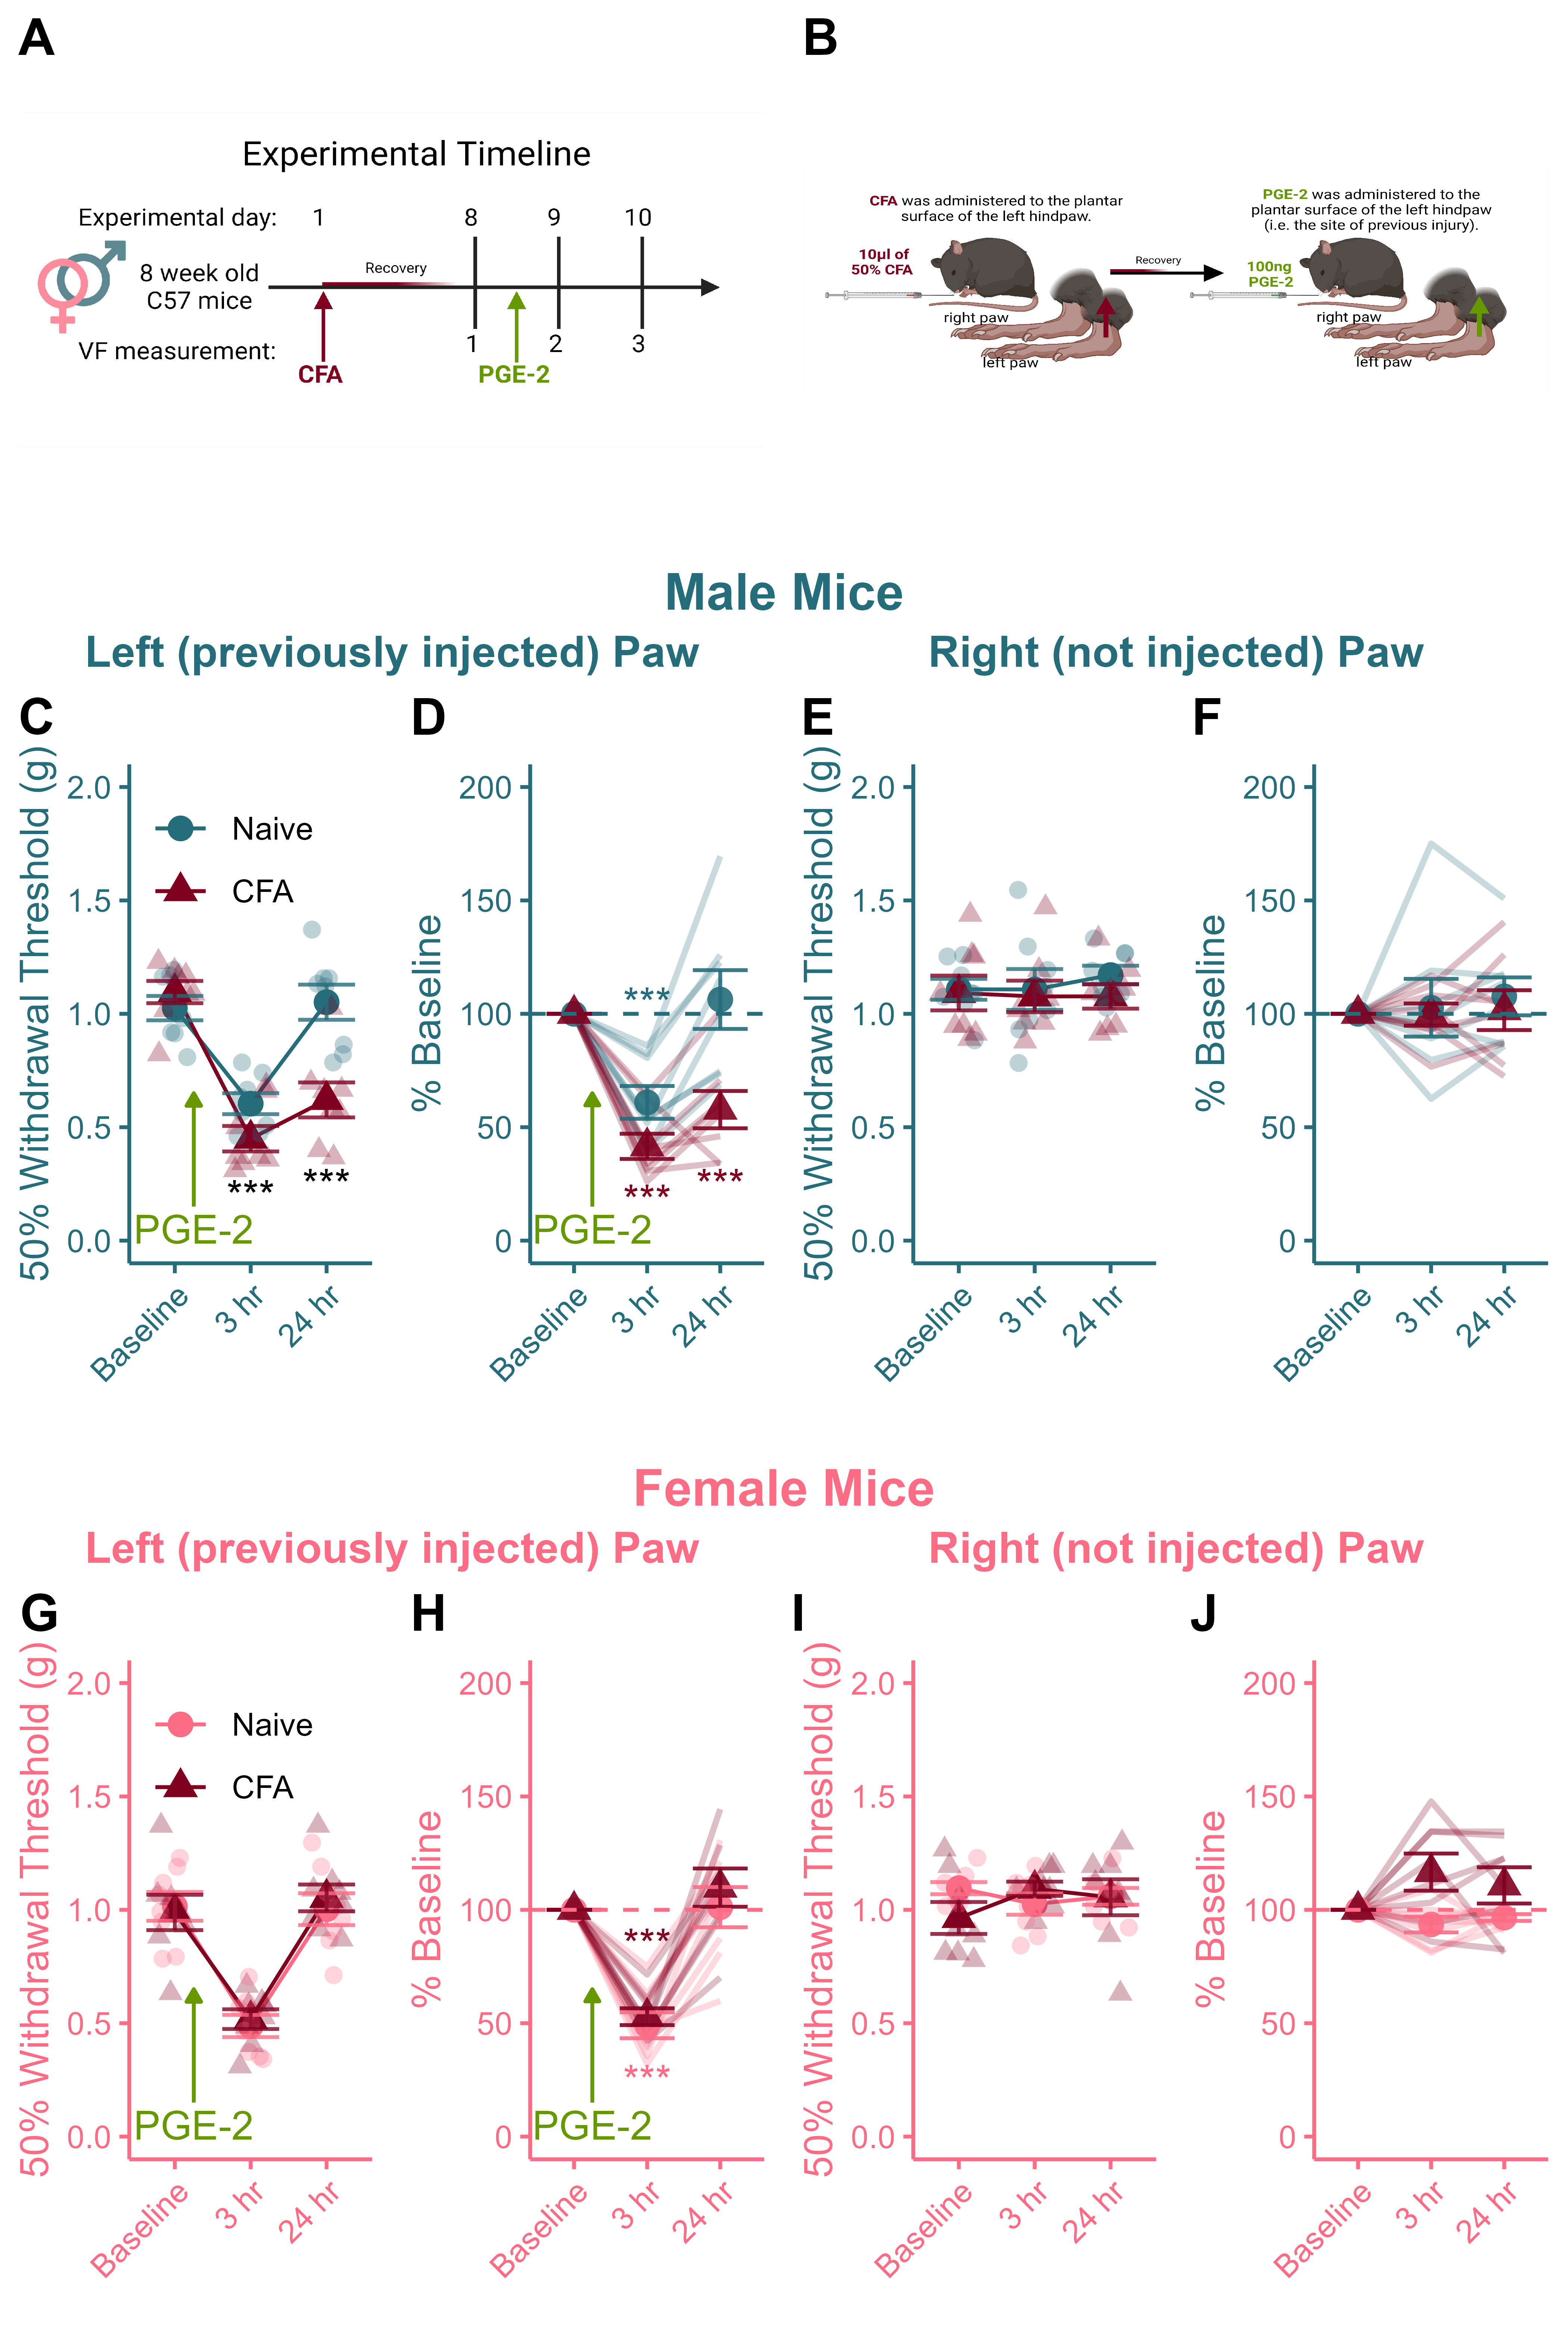
\includegraphics[width=58.33in]{Figs/4_CFA_PGE2} \end{center}

\textbf{Figure 4.} \emph{CFA-priming produced enhanced and prolonged mechanical sensitivity after PGE-2 injection in male mice only.} (A) Timeline of experimental testing. (B) PGE-2 was administered to the site of previous injury to test expression of pain sensitization. CFA-primed male mice exhibited enhanced (3hr) and prolonged (24hr) mechanical sensitivity after PGE-2 injection relative to naive mice injected with PGE-2 (C). naive males recovered their baseline paw withdrawal thresholds 24 hours after PGE-2, whereas CFA-primed males exhibited ongoing sensitivity (C,D). There was no difference in the magnitude of mechanical sensitivity induced by PGE-2 injection 3hrs post administration in female mice (G), and both CFA-primed and pin-naive mice recovered basal levels of mechanical sensitivity 24 hours post-administration (H). There were no decreases in paw sensitivity in the contralateral (never-injected) paw during pain \& recovery from PGE-2 administration (E,F,I,J). Data expressed as mean +/- SEM. \(***\) Indicates between-group difference where \emph{p} \textless{} 0.001 and \# indicates a within-subject difference from baseline where \emph{p} \textless0.05.

\hypertarget{statistics}{%
\section*{Statistics}\label{statistics}}
\addcontentsline{toc}{section}{Statistics}

\begin{Shaded}
\begin{Highlighting}[]
\CommentTok{\# Select the left paws}
\NormalTok{left\_paws }\OtherTok{\textless{}{-}} \FunctionTok{rbind}\NormalTok{(L\_Male,L\_Female)}

\CommentTok{\# Remove those that did not receive PGE2 and switch to long form}
\NormalTok{a }\OtherTok{\textless{}{-}}\NormalTok{ left\_paws }\SpecialCharTok{\%\textgreater{}\%}
  \FunctionTok{filter}\NormalTok{(PGE2 }\SpecialCharTok{==} \StringTok{"PGE2"}\NormalTok{) }\SpecialCharTok{\%\textgreater{}\%}
  \FunctionTok{melt}\NormalTok{(}\AttributeTok{id.vars=}\FunctionTok{c}\NormalTok{(}\StringTok{"ID"}\NormalTok{,}\StringTok{"CFA"}\NormalTok{,}\StringTok{"Sex"}\NormalTok{,}\StringTok{"PGE2"}\NormalTok{))}

\CommentTok{\# Run 3{-}way ANOVA: Sex X CFA X Day of testing (VF)}
\NormalTok{b }\OtherTok{\textless{}{-}} \FunctionTok{anova\_test}\NormalTok{(}\AttributeTok{data=}\NormalTok{a,}\AttributeTok{dv=}\NormalTok{value,}\AttributeTok{between=}\FunctionTok{c}\NormalTok{(Sex,CFA),}\AttributeTok{within=}\NormalTok{variable,}\AttributeTok{wid=}\NormalTok{ID)}
\NormalTok{knitr}\SpecialCharTok{::}\FunctionTok{kable}\NormalTok{(}\FunctionTok{get\_anova\_table}\NormalTok{(b))}
\end{Highlighting}
\end{Shaded}

\begin{tabular}{l|r|r|r|r|l|r}
\hline
Effect & DFn & DFd & F & p & p<.05 & ges\\
\hline
Sex & 1 & 28 & 1.154 & 0.292 &  & 0.014\\
\hline
CFA & 1 & 28 & 5.116 & 0.032 & * & 0.060\\
\hline
variable & 2 & 56 & 93.042 & 0.000 & * & 0.684\\
\hline
Sex:CFA & 1 & 28 & 7.754 & 0.010 & * & 0.088\\
\hline
Sex:variable & 2 & 56 & 5.705 & 0.006 & * & 0.117\\
\hline
CFA:variable & 2 & 56 & 3.548 & 0.035 & * & 0.076\\
\hline
Sex:CFA:variable & 2 & 56 & 6.479 & 0.003 & * & 0.131\\
\hline
\end{tabular}

\begin{Shaded}
\begin{Highlighting}[]
\CommentTok{\# Run both sets of follow ups: }

\DocumentationTok{\#\# Effect of CFA on each day of testing split by sex}
\NormalTok{b }\OtherTok{\textless{}{-}}\NormalTok{ a }\SpecialCharTok{\%\textgreater{}\%}
  \FunctionTok{group\_by}\NormalTok{(Sex,variable) }\SpecialCharTok{\%\textgreater{}\%}
  \FunctionTok{pairwise\_t\_test}\NormalTok{(value}\SpecialCharTok{\textasciitilde{}}\NormalTok{CFA)}

\FunctionTok{tt}\NormalTok{(b)}
\end{Highlighting}
\end{Shaded}

\begin{table}
\centering
\begin{tblr}[         %% tabularray outer open
]                     %% tabularray outer close
{                     %% tabularray inner open
colspec={Q[]Q[]Q[]Q[]Q[]Q[]Q[]Q[]Q[]Q[]Q[]},
}                     %% tabularray inner close
\toprule
Sex & variable & .y. & group1 & group2 & n1 & n2 & p & p.signif & p.adj & p.adj.signif \\ \midrule %% TinyTableHeader
Female & Baseline & value & Naive & CFA & 8 & 8 & 0.77900 & ns  & 0.77900 & ns  \\
Female & 3 hr     & value & Naive & CFA & 8 & 8 & 0.62900 & ns  & 0.62900 & ns  \\
Female & 24 hr    & value & Naive & CFA & 8 & 8 & 0.57000 & ns  & 0.57000 & ns  \\
Male   & Baseline & value & Naive & CFA & 8 & 8 & 0.31600 & ns  & 0.31600 & ns  \\
Male   & 3 hr     & value & Naive & CFA & 8 & 8 & 0.03960 & *   & 0.03960 & *   \\
Male   & 24 hr    & value & Naive & CFA & 8 & 8 & 0.00087 & *** & 0.00087 & *** \\
\bottomrule
\end{tblr}
\end{table}

\begin{Shaded}
\begin{Highlighting}[]
\DocumentationTok{\#\# Effect of Sex on each day of testing split by CFA history}
\NormalTok{c }\OtherTok{\textless{}{-}}\NormalTok{ a }\SpecialCharTok{\%\textgreater{}\%}
  \FunctionTok{group\_by}\NormalTok{(CFA,variable) }\SpecialCharTok{\%\textgreater{}\%}
  \FunctionTok{pairwise\_t\_test}\NormalTok{(value}\SpecialCharTok{\textasciitilde{}}\NormalTok{Sex)}

\FunctionTok{tt}\NormalTok{(c)}
\end{Highlighting}
\end{Shaded}

\begin{table}
\centering
\begin{tblr}[         %% tabularray outer open
]                     %% tabularray outer close
{                     %% tabularray inner open
colspec={Q[]Q[]Q[]Q[]Q[]Q[]Q[]Q[]Q[]Q[]Q[]},
}                     %% tabularray inner close
\toprule
CFA & variable & .y. & group1 & group2 & n1 & n2 & p & p.signif & p.adj & p.adj.signif \\ \midrule %% TinyTableHeader
Naive & Baseline & value & Female & Male & 8 & 8 & 0.901000 & ns  & 0.901000 & ns  \\
Naive & 3 hr     & value & Female & Male & 8 & 8 & 0.086800 & ns  & 0.086800 & ns  \\
Naive & 24 hr    & value & Female & Male & 8 & 8 & 0.628000 & ns  & 0.628000 & ns  \\
CFA   & Baseline & value & Female & Male & 8 & 8 & 0.232000 & ns  & 0.232000 & ns  \\
CFA   & 3 hr     & value & Female & Male & 8 & 8 & 0.319000 & ns  & 0.319000 & ns  \\
CFA   & 24 hr    & value & Female & Male & 8 & 8 & 0.000306 & *** & 0.000306 & *** \\
\bottomrule
\end{tblr}
\end{table}

\begin{Shaded}
\begin{Highlighting}[]
\DocumentationTok{\#\# Effect of DAY within each group}
\NormalTok{d }\OtherTok{\textless{}{-}}\NormalTok{ a }\SpecialCharTok{\%\textgreater{}\%}
  \FunctionTok{group\_by}\NormalTok{(CFA,Sex) }\SpecialCharTok{\%\textgreater{}\%}
  \FunctionTok{pairwise\_t\_test}\NormalTok{(value}\SpecialCharTok{\textasciitilde{}}\NormalTok{variable,}\AttributeTok{p.adjust.method =} \StringTok{"bonferroni"}\NormalTok{)}

\FunctionTok{tt}\NormalTok{(d)}
\end{Highlighting}
\end{Shaded}

\begin{table}
\centering
\begin{tblr}[         %% tabularray outer open
]                     %% tabularray outer close
{                     %% tabularray inner open
colspec={Q[]Q[]Q[]Q[]Q[]Q[]Q[]Q[]Q[]Q[]Q[]},
}                     %% tabularray inner close
\toprule
CFA & Sex & .y. & group1 & group2 & n1 & n2 & p & p.signif & p.adj & p.adj.signif \\ \midrule %% TinyTableHeader
Naive & Female & value & Baseline & 3 hr  & 8 & 8 & 0.000002010 & **** & 0.000006040 & **** \\
Naive & Female & value & Baseline & 24 hr & 8 & 8 & 0.879000000 & ns   & 1.000000000 & ns   \\
Naive & Female & value & 3 hr     & 24 hr & 8 & 8 & 0.000002830 & **** & 0.000008490 & **** \\
Naive & Male   & value & Baseline & 3 hr  & 8 & 8 & 0.000033200 & **** & 0.000099500 & **** \\
Naive & Male   & value & Baseline & 24 hr & 8 & 8 & 0.748000000 & ns   & 1.000000000 & ns   \\
Naive & Male   & value & 3 hr     & 24 hr & 8 & 8 & 0.000015600 & **** & 0.000046700 & **** \\
CFA   & Female & value & Baseline & 3 hr  & 8 & 8 & 0.000010300 & **** & 0.000030900 & **** \\
CFA   & Female & value & Baseline & 24 hr & 8 & 8 & 0.441000000 & ns   & 1.000000000 & ns   \\
CFA   & Female & value & 3 hr     & 24 hr & 8 & 8 & 0.000001760 & **** & 0.000005290 & **** \\
CFA   & Male   & value & Baseline & 3 hr  & 8 & 8 & 0.000000103 & **** & 0.000000308 & **** \\
CFA   & Male   & value & Baseline & 24 hr & 8 & 8 & 0.000009240 & **** & 0.000027700 & **** \\
CFA   & Male   & value & 3 hr     & 24 hr & 8 & 8 & 0.049300000 & *    & 0.148000000 & ns   \\
\bottomrule
\end{tblr}
\end{table}

\hypertarget{figure-5---recovery-from-footshock}{%
\chapter*{Figure 5 - Recovery From Footshock}\label{figure-5---recovery-from-footshock}}
\addcontentsline{toc}{chapter}{Figure 5 - Recovery From Footshock}

\hypertarget{published-image-4}{%
\section*{Published Image}\label{published-image-4}}
\addcontentsline{toc}{section}{Published Image}

\begin{center}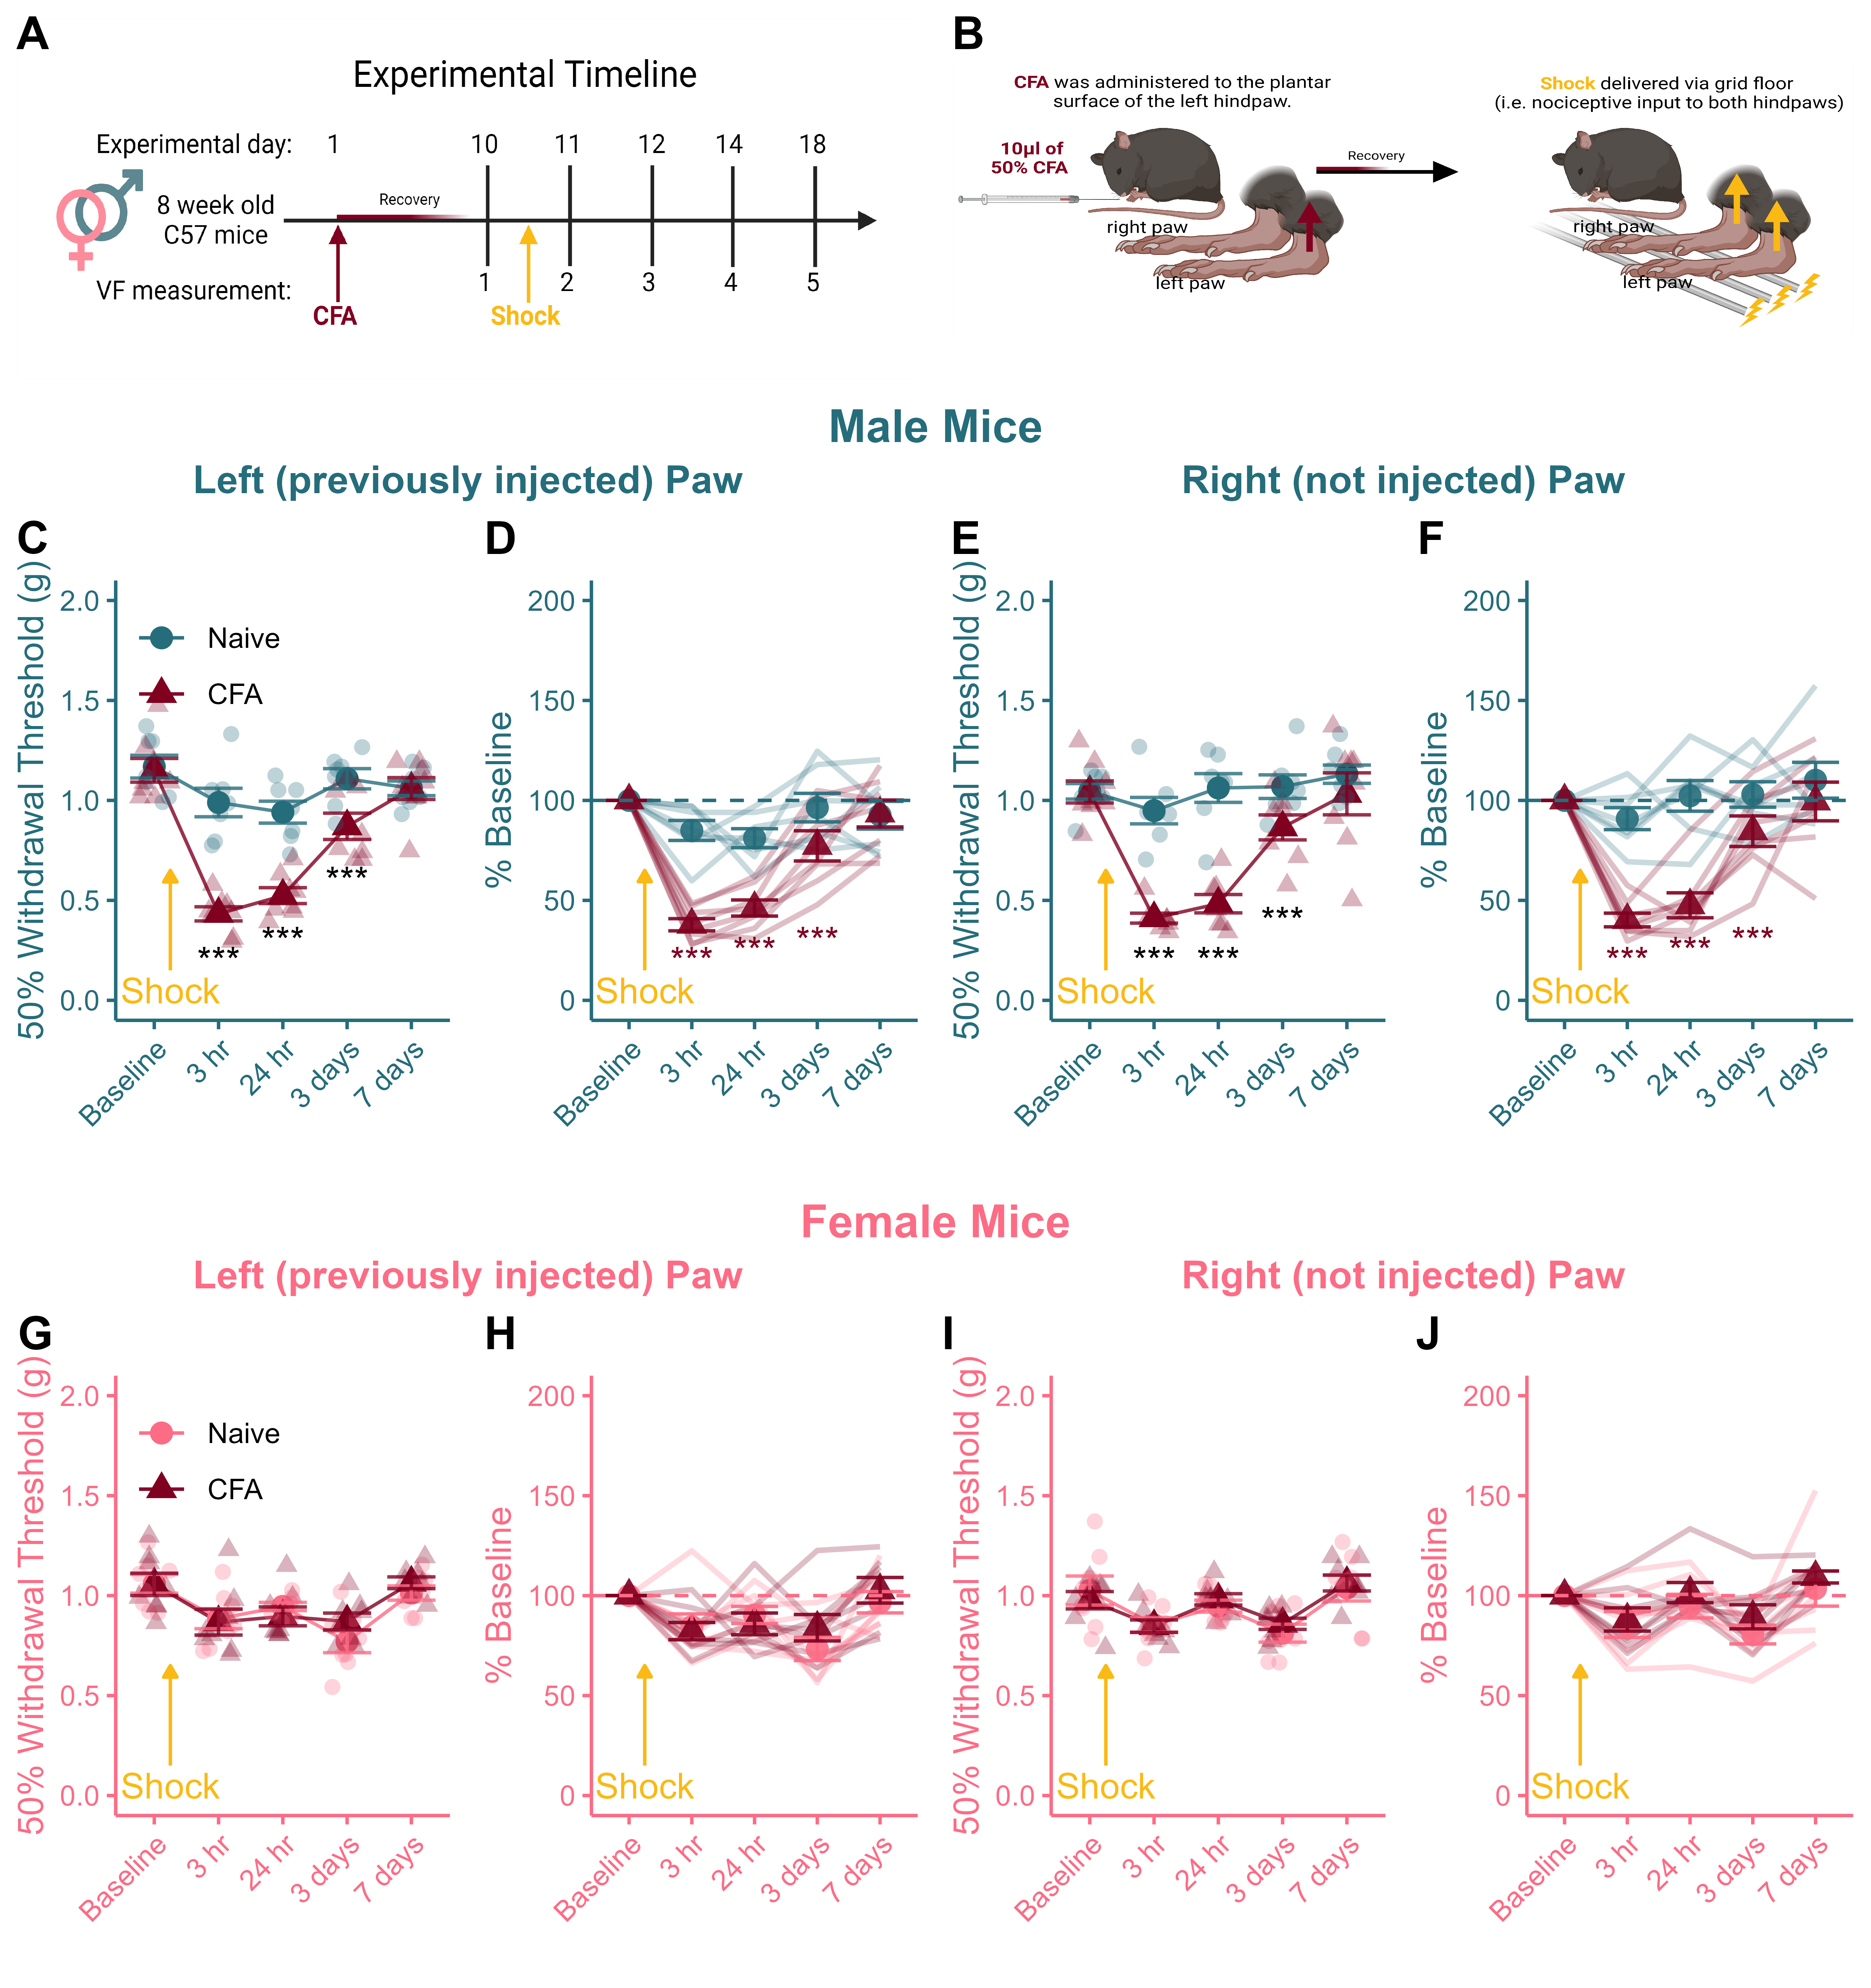
\includegraphics[width=77.78in]{Figs/5_Shock_VF} \end{center}

\textbf{Figure 5.} \emph{CFA-priming enhances mechanical sensitivity induced by electrical footshock in the previously injured and the contralateral hind paw in males (and not females).} (A) Timeline of experimental testing (B) Footshock was simultaneously delivered to the site of the previous injury and the contralateral hindpaw. CFA-primed male mice exhibited enhanced mechanical sensitivity after footshock in both the left (C, D) and the right (E, F) hind paws relative to mice that had undergone fear conditioning but had not been subjected to a previous injury. There was no effect of CFA-priming on shock-induced mechanical sensitivity among female mice (G-J). Data expressed as mean +/- SEM. \(***\) Indicates a between-group difference where \emph{p} \textless{} 0.05 and \# indicates a within-subject difference from baseline where \emph{p} \textless{} 0.05.

\hypertarget{statistics-1}{%
\section*{Statistics}\label{statistics-1}}
\addcontentsline{toc}{section}{Statistics}

\hypertarget{left-paws}{%
\subsection*{Left Paws}\label{left-paws}}
\addcontentsline{toc}{subsection}{Left Paws}

\begin{Shaded}
\begin{Highlighting}[]
\NormalTok{L\_Male}\SpecialCharTok{$}\NormalTok{Sex }\OtherTok{\textless{}{-}} \StringTok{"Male"}
\NormalTok{L\_Female}\SpecialCharTok{$}\NormalTok{Sex }\OtherTok{\textless{}{-}} \StringTok{"Female"}

\CommentTok{\# Select the left paws}
\NormalTok{left\_paws }\OtherTok{\textless{}{-}} \FunctionTok{rbind}\NormalTok{(L\_Male,L\_Female)}

\CommentTok{\# Switch to long form}
\NormalTok{a }\OtherTok{\textless{}{-}}\NormalTok{ left\_paws }\SpecialCharTok{\%\textgreater{}\%}
  \FunctionTok{melt}\NormalTok{(}\AttributeTok{id.vars=}\FunctionTok{c}\NormalTok{(}\StringTok{"ID"}\NormalTok{,}\StringTok{"CFA"}\NormalTok{,}\StringTok{"Sex"}\NormalTok{))}

\CommentTok{\# Run 3{-}way ANOVA: Sex X CFA X Day of testing (VF)}
\NormalTok{b }\OtherTok{\textless{}{-}} \FunctionTok{anova\_test}\NormalTok{(}\AttributeTok{data=}\NormalTok{a,}\AttributeTok{dv=}\NormalTok{value,}\AttributeTok{between=}\FunctionTok{c}\NormalTok{(Sex,CFA),}\AttributeTok{within=}\NormalTok{variable,}\AttributeTok{wid=}\NormalTok{ID)}
\NormalTok{knitr}\SpecialCharTok{::}\FunctionTok{kable}\NormalTok{(}\FunctionTok{get\_anova\_table}\NormalTok{(b))}
\end{Highlighting}
\end{Shaded}

\begin{tabular}{l|r|r|r|r|l|r}
\hline
Effect & DFn & DFd & F & p & p<.05 & ges\\
\hline
Sex & 1 & 27 & 0.251 & 0.6200000 &  & 0.002\\
\hline
CFA & 1 & 27 & 22.366 & 0.0000631 & * & 0.177\\
\hline
variable & 4 & 108 & 36.017 & 0.0000000 & * & 0.497\\
\hline
Sex:CFA & 1 & 27 & 29.188 & 0.0000103 & * & 0.219\\
\hline
Sex:variable & 4 & 108 & 12.032 & 0.0000000 & * & 0.248\\
\hline
CFA:variable & 4 & 108 & 9.054 & 0.0000024 & * & 0.199\\
\hline
Sex:CFA:variable & 4 & 108 & 5.894 & 0.0002500 & * & 0.139\\
\hline
\end{tabular}

\begin{Shaded}
\begin{Highlighting}[]
\CommentTok{\# Run both sets of follow ups: }

\DocumentationTok{\#\# Effect of CFA on each day of testing split by sex}
\NormalTok{b }\OtherTok{\textless{}{-}}\NormalTok{ a }\SpecialCharTok{\%\textgreater{}\%}
  \FunctionTok{group\_by}\NormalTok{(Sex,variable) }\SpecialCharTok{\%\textgreater{}\%}
  \FunctionTok{pairwise\_t\_test}\NormalTok{(value}\SpecialCharTok{\textasciitilde{}}\NormalTok{CFA)}

\FunctionTok{tt}\NormalTok{(b)}
\end{Highlighting}
\end{Shaded}

\begin{table}
\centering
\begin{tblr}[         %% tabularray outer open
]                     %% tabularray outer close
{                     %% tabularray inner open
colspec={Q[]Q[]Q[]Q[]Q[]Q[]Q[]Q[]Q[]Q[]Q[]},
}                     %% tabularray inner close
\toprule
Sex & variable & .y. & group1 & group2 & n1 & n2 & p & p.signif & p.adj & p.adj.signif \\ \midrule %% TinyTableHeader
Female & Baseline & value & Naive & CFA & 8 & 8 & 0.96400000 & ns   & 0.96400000 & ns   \\
Female & 3 hr     & value & Naive & CFA & 8 & 8 & 0.82300000 & ns   & 0.82300000 & ns   \\
Female & 24 hr    & value & Naive & CFA & 8 & 8 & 0.32200000 & ns   & 0.32200000 & ns   \\
Female & 3 days   & value & Naive & CFA & 8 & 8 & 0.14700000 & ns   & 0.14700000 & ns   \\
Female & 7 days   & value & Naive & CFA & 8 & 8 & 0.25400000 & ns   & 0.25400000 & ns   \\
Male   & Baseline & value & Naive & CFA & 7 & 8 & 0.82100000 & ns   & 0.82100000 & ns   \\
Male   & 3 hr     & value & Naive & CFA & 7 & 8 & 0.00000518 & **** & 0.00000518 & **** \\
Male   & 24 hr    & value & Naive & CFA & 7 & 8 & 0.00002210 & **** & 0.00002210 & **** \\
Male   & 3 days   & value & Naive & CFA & 7 & 8 & 0.01170000 & *    & 0.01170000 & *    \\
Male   & 7 days   & value & Naive & CFA & 7 & 8 & 0.98500000 & ns   & 0.98500000 & ns   \\
\bottomrule
\end{tblr}
\end{table}

\begin{Shaded}
\begin{Highlighting}[]
\DocumentationTok{\#\# Effect of Sex on each day of testing split by CFA history}
\NormalTok{c }\OtherTok{\textless{}{-}}\NormalTok{ a }\SpecialCharTok{\%\textgreater{}\%}
  \FunctionTok{group\_by}\NormalTok{(CFA,variable) }\SpecialCharTok{\%\textgreater{}\%}
  \FunctionTok{pairwise\_t\_test}\NormalTok{(value}\SpecialCharTok{\textasciitilde{}}\NormalTok{Sex)}

\FunctionTok{tt}\NormalTok{(c)}
\end{Highlighting}
\end{Shaded}

\begin{table}
\centering
\begin{tblr}[         %% tabularray outer open
]                     %% tabularray outer close
{                     %% tabularray inner open
colspec={Q[]Q[]Q[]Q[]Q[]Q[]Q[]Q[]Q[]Q[]Q[]},
}                     %% tabularray inner close
\toprule
CFA & variable & .y. & group1 & group2 & n1 & n2 & p & p.signif & p.adj & p.adj.signif \\ \midrule %% TinyTableHeader
Naive & Baseline & value & Female & Male & 8 & 7 & 0.1470000 & ns   & 0.1470000 & ns   \\
Naive & 3 hr     & value & Female & Male & 8 & 7 & 0.2300000 & ns   & 0.2300000 & ns   \\
Naive & 24 hr    & value & Female & Male & 8 & 7 & 0.9360000 & ns   & 0.9360000 & ns   \\
Naive & 3 days   & value & Female & Male & 8 & 7 & 0.0004790 & ***  & 0.0004790 & ***  \\
Naive & 7 days   & value & Female & Male & 8 & 7 & 0.3520000 & ns   & 0.3520000 & ns   \\
CFA   & Baseline & value & Female & Male & 8 & 8 & 0.2360000 & ns   & 0.2360000 & ns   \\
CFA   & 3 hr     & value & Female & Male & 8 & 8 & 0.0000190 & **** & 0.0000190 & **** \\
CFA   & 24 hr    & value & Female & Male & 8 & 8 & 0.0000155 & **** & 0.0000155 & **** \\
CFA   & 3 days   & value & Female & Male & 8 & 8 & 0.9980000 & ns   & 0.9980000 & ns   \\
CFA   & 7 days   & value & Female & Male & 8 & 8 & 0.9330000 & ns   & 0.9330000 & ns   \\
\bottomrule
\end{tblr}
\end{table}

\begin{Shaded}
\begin{Highlighting}[]
\DocumentationTok{\#\# Effect of DAY within each group}
\NormalTok{d }\OtherTok{\textless{}{-}}\NormalTok{ a }\SpecialCharTok{\%\textgreater{}\%}
  \FunctionTok{group\_by}\NormalTok{(CFA,Sex) }\SpecialCharTok{\%\textgreater{}\%}
  \FunctionTok{pairwise\_t\_test}\NormalTok{(value}\SpecialCharTok{\textasciitilde{}}\NormalTok{variable,}\AttributeTok{p.adjust.method =} \StringTok{"bonferroni"}\NormalTok{)}

\FunctionTok{tt}\NormalTok{(d)}
\end{Highlighting}
\end{Shaded}

\begin{table}
\centering
\begin{tblr}[         %% tabularray outer open
]                     %% tabularray outer close
{                     %% tabularray inner open
colspec={Q[]Q[]Q[]Q[]Q[]Q[]Q[]Q[]Q[]Q[]Q[]},
}                     %% tabularray inner close
\toprule
CFA & Sex & .y. & group1 & group2 & n1 & n2 & p & p.signif & p.adj & p.adj.signif \\ \midrule %% TinyTableHeader
Naive & Female & value & Baseline & 3 hr   & 8 & 8 & 0.00468000000000 & **   & 0.0468000000000 & *    \\
Naive & Female & value & Baseline & 24 hr  & 8 & 8 & 0.05740000000000 & ns   & 0.5740000000000 & ns   \\
Naive & Female & value & 3 hr     & 24 hr  & 8 & 8 & 0.29800000000000 & ns   & 1.0000000000000 & ns   \\
Naive & Female & value & Baseline & 3 days & 8 & 8 & 0.00001600000000 & **** & 0.0001600000000 & ***  \\
Naive & Female & value & 3 hr     & 3 days & 8 & 8 & 0.05580000000000 & ns   & 0.5580000000000 & ns   \\
Naive & Female & value & 24 hr    & 3 days & 8 & 8 & 0.00452000000000 & **   & 0.0452000000000 & *    \\
Naive & Female & value & Baseline & 7 days & 8 & 8 & 0.42600000000000 & ns   & 1.0000000000000 & ns   \\
Naive & Female & value & 3 hr     & 7 days & 8 & 8 & 0.03320000000000 & *    & 0.3320000000000 & ns   \\
Naive & Female & value & 24 hr    & 7 days & 8 & 8 & 0.25400000000000 & ns   & 1.0000000000000 & ns   \\
Naive & Female & value & 3 days   & 7 days & 8 & 8 & 0.00017700000000 & ***  & 0.0017700000000 & **   \\
Naive & Male   & value & Baseline & 3 hr   & 7 & 7 & 0.02860000000000 & *    & 0.2860000000000 & ns   \\
Naive & Male   & value & Baseline & 24 hr  & 7 & 7 & 0.00662000000000 & **   & 0.0662000000000 & ns   \\
Naive & Male   & value & 3 hr     & 24 hr  & 7 & 7 & 0.54100000000000 & ns   & 1.0000000000000 & ns   \\
Naive & Male   & value & Baseline & 3 days & 7 & 7 & 0.44400000000000 & ns   & 1.0000000000000 & ns   \\
Naive & Male   & value & 3 hr     & 3 days & 7 & 7 & 0.13800000000000 & ns   & 1.0000000000000 & ns   \\
Naive & Male   & value & 24 hr    & 3 days & 7 & 7 & 0.04040000000000 & *    & 0.4040000000000 & ns   \\
Naive & Male   & value & Baseline & 7 days & 7 & 7 & 0.17500000000000 & ns   & 1.0000000000000 & ns   \\
Naive & Male   & value & 3 hr     & 7 days & 7 & 7 & 0.37000000000000 & ns   & 1.0000000000000 & ns   \\
Naive & Male   & value & 24 hr    & 7 days & 7 & 7 & 0.13700000000000 & ns   & 1.0000000000000 & ns   \\
Naive & Male   & value & 3 days   & 7 days & 7 & 7 & 0.54400000000000 & ns   & 1.0000000000000 & ns   \\
CFA   & Female & value & Baseline & 3 hr   & 8 & 8 & 0.00645000000000 & **   & 0.0645000000000 & ns   \\
CFA   & Female & value & Baseline & 24 hr  & 8 & 8 & 0.01930000000000 & *    & 0.1930000000000 & ns   \\
CFA   & Female & value & 3 hr     & 24 hr  & 8 & 8 & 0.65900000000000 & ns   & 1.0000000000000 & ns   \\
CFA   & Female & value & Baseline & 3 days & 8 & 8 & 0.00735000000000 & **   & 0.0735000000000 & ns   \\
CFA   & Female & value & 3 hr     & 3 days & 8 & 8 & 0.95900000000000 & ns   & 1.0000000000000 & ns   \\
CFA   & Female & value & 24 hr    & 3 days & 8 & 8 & 0.69600000000000 & ns   & 1.0000000000000 & ns   \\
CFA   & Female & value & Baseline & 7 days & 8 & 8 & 0.90100000000000 & ns   & 1.0000000000000 & ns   \\
CFA   & Female & value & 3 hr     & 7 days & 8 & 8 & 0.00467000000000 & **   & 0.0467000000000 & *    \\
CFA   & Female & value & 24 hr    & 7 days & 8 & 8 & 0.01430000000000 & *    & 0.1430000000000 & ns   \\
CFA   & Female & value & 3 days   & 7 days & 8 & 8 & 0.00534000000000 & **   & 0.0534000000000 & ns   \\
CFA   & Male   & value & Baseline & 3 hr   & 8 & 8 & 0.00000000000326 & **** & 0.0000000000326 & **** \\
CFA   & Male   & value & Baseline & 24 hr  & 8 & 8 & 0.00000000010800 & **** & 0.0000000010800 & **** \\
CFA   & Male   & value & 3 hr     & 24 hr  & 8 & 8 & 0.19600000000000 & ns   & 1.0000000000000 & ns   \\
CFA   & Male   & value & Baseline & 3 days & 8 & 8 & 0.00027300000000 & ***  & 0.0027300000000 & **   \\
CFA   & Male   & value & 3 hr     & 3 days & 8 & 8 & 0.00000029100000 & **** & 0.0000029100000 & **** \\
CFA   & Male   & value & 24 hr    & 3 days & 8 & 8 & 0.00001580000000 & **** & 0.0001580000000 & ***  \\
CFA   & Male   & value & Baseline & 7 days & 8 & 8 & 0.19600000000000 & ns   & 1.0000000000000 & ns   \\
CFA   & Male   & value & 3 hr     & 7 days & 8 & 8 & 0.00000000010800 & **** & 0.0000000010800 & **** \\
CFA   & Male   & value & 24 hr    & 7 days & 8 & 8 & 0.00000000444000 & **** & 0.0000000444000 & **** \\
CFA   & Male   & value & 3 days   & 7 days & 8 & 8 & 0.00989000000000 & **   & 0.0989000000000 & ns   \\
\bottomrule
\end{tblr}
\end{table}

\hypertarget{right-paws}{%
\subsection*{Right Paws}\label{right-paws}}
\addcontentsline{toc}{subsection}{Right Paws}

\begin{Shaded}
\begin{Highlighting}[]
\NormalTok{R\_Male}\SpecialCharTok{$}\NormalTok{Sex }\OtherTok{\textless{}{-}} \StringTok{"Male"}
\NormalTok{R\_Female}\SpecialCharTok{$}\NormalTok{Sex }\OtherTok{\textless{}{-}} \StringTok{"Female"}

\CommentTok{\# Select the right paws}
\NormalTok{right\_paws }\OtherTok{\textless{}{-}} \FunctionTok{rbind}\NormalTok{(R\_Male,R\_Female)}

\CommentTok{\# Switch to long form}
\NormalTok{a }\OtherTok{\textless{}{-}}\NormalTok{ right\_paws }\SpecialCharTok{\%\textgreater{}\%}
  \FunctionTok{melt}\NormalTok{(}\AttributeTok{id.vars=}\FunctionTok{c}\NormalTok{(}\StringTok{"ID"}\NormalTok{,}\StringTok{"CFA"}\NormalTok{,}\StringTok{"Sex"}\NormalTok{))}

\CommentTok{\# Run 3{-}way ANOVA: Sex X CFA X Day of testing (VF)}
\NormalTok{b }\OtherTok{\textless{}{-}} \FunctionTok{anova\_test}\NormalTok{(}\AttributeTok{data=}\NormalTok{a,}\AttributeTok{dv=}\NormalTok{value,}\AttributeTok{between=}\FunctionTok{c}\NormalTok{(Sex,CFA),}\AttributeTok{within=}\NormalTok{variable,}\AttributeTok{wid=}\NormalTok{ID)}
\NormalTok{knitr}\SpecialCharTok{::}\FunctionTok{kable}\NormalTok{(}\FunctionTok{get\_anova\_table}\NormalTok{(b))}
\end{Highlighting}
\end{Shaded}

\begin{tabular}{l|r|r|r|r|l|r}
\hline
Effect & DFn & DFd & F & p & p<.05 & ges\\
\hline
Sex & 1 & 27 & 1.484 & 0.2340000 &  & 0.014\\
\hline
CFA & 1 & 27 & 28.665 & 0.0000118 & * & 0.213\\
\hline
variable & 4 & 108 & 24.583 & 0.0000000 & * & 0.404\\
\hline
Sex:CFA & 1 & 27 & 32.973 & 0.0000042 & * & 0.238\\
\hline
Sex:variable & 4 & 108 & 8.449 & 0.0000057 & * & 0.189\\
\hline
CFA:variable & 4 & 108 & 6.520 & 0.0000972 & * & 0.152\\
\hline
Sex:CFA:variable & 4 & 108 & 7.949 & 0.0000118 & * & 0.180\\
\hline
\end{tabular}

\begin{Shaded}
\begin{Highlighting}[]
\CommentTok{\# Run both sets of follow ups: }

\DocumentationTok{\#\# Effect of CFA on each day of testing split by sex}
\NormalTok{b }\OtherTok{\textless{}{-}}\NormalTok{ a }\SpecialCharTok{\%\textgreater{}\%}
  \FunctionTok{group\_by}\NormalTok{(Sex,variable) }\SpecialCharTok{\%\textgreater{}\%}
  \FunctionTok{pairwise\_t\_test}\NormalTok{(value}\SpecialCharTok{\textasciitilde{}}\NormalTok{CFA)}

\FunctionTok{tt}\NormalTok{(b)}
\end{Highlighting}
\end{Shaded}

\begin{table}
\centering
\begin{tblr}[         %% tabularray outer open
]                     %% tabularray outer close
{                     %% tabularray inner open
colspec={Q[]Q[]Q[]Q[]Q[]Q[]Q[]Q[]Q[]Q[]Q[]},
}                     %% tabularray inner close
\toprule
Sex & variable & .y. & group1 & group2 & n1 & n2 & p & p.signif & p.adj & p.adj.signif \\ \midrule %% TinyTableHeader
Female & Baseline & value & Naive & CFA & 8 & 8 & 0.54900000 & ns   & 0.54900000 & ns   \\
Female & 3 hr     & value & Naive & CFA & 8 & 8 & 0.88500000 & ns   & 0.88500000 & ns   \\
Female & 24 hr    & value & Naive & CFA & 8 & 8 & 0.39700000 & ns   & 0.39700000 & ns   \\
Female & 3 days   & value & Naive & CFA & 8 & 8 & 0.36000000 & ns   & 0.36000000 & ns   \\
Female & 7 days   & value & Naive & CFA & 8 & 8 & 0.74000000 & ns   & 0.74000000 & ns   \\
Male   & Baseline & value & Naive & CFA & 7 & 8 & 0.96300000 & ns   & 0.96300000 & ns   \\
Male   & 3 hr     & value & Naive & CFA & 7 & 8 & 0.00000193 & **** & 0.00000193 & **** \\
Male   & 24 hr    & value & Naive & CFA & 7 & 8 & 0.00000781 & **** & 0.00000781 & **** \\
Male   & 3 days   & value & Naive & CFA & 7 & 8 & 0.02970000 & *    & 0.02970000 & *    \\
Male   & 7 days   & value & Naive & CFA & 7 & 8 & 0.40400000 & ns   & 0.40400000 & ns   \\
\bottomrule
\end{tblr}
\end{table}

\begin{Shaded}
\begin{Highlighting}[]
\DocumentationTok{\#\# Effect of Sex on each day of testing split by CFA history}
\NormalTok{c }\OtherTok{\textless{}{-}}\NormalTok{ a }\SpecialCharTok{\%\textgreater{}\%}
  \FunctionTok{group\_by}\NormalTok{(CFA,variable) }\SpecialCharTok{\%\textgreater{}\%}
  \FunctionTok{pairwise\_t\_test}\NormalTok{(value}\SpecialCharTok{\textasciitilde{}}\NormalTok{Sex)}

\FunctionTok{tt}\NormalTok{(c)}
\end{Highlighting}
\end{Shaded}

\begin{table}
\centering
\begin{tblr}[         %% tabularray outer open
]                     %% tabularray outer close
{                     %% tabularray inner open
colspec={Q[]Q[]Q[]Q[]Q[]Q[]Q[]Q[]Q[]Q[]Q[]},
}                     %% tabularray inner close
\toprule
CFA & variable & .y. & group1 & group2 & n1 & n2 & p & p.signif & p.adj & p.adj.signif \\ \midrule %% TinyTableHeader
Naive & Baseline & value & Female & Male & 8 & 7 & 0.8090000000 & ns   & 0.8090000000 & ns   \\
Naive & 3 hr     & value & Female & Male & 8 & 7 & 0.2030000000 & ns   & 0.2030000000 & ns   \\
Naive & 24 hr    & value & Female & Male & 8 & 7 & 0.1420000000 & ns   & 0.1420000000 & ns   \\
Naive & 3 days   & value & Female & Male & 8 & 7 & 0.0031500000 & **   & 0.0031500000 & **   \\
Naive & 7 days   & value & Female & Male & 8 & 7 & 0.2580000000 & ns   & 0.2580000000 & ns   \\
CFA   & Baseline & value & Female & Male & 8 & 8 & 0.3350000000 & ns   & 0.3350000000 & ns   \\
CFA   & 3 hr     & value & Female & Male & 8 & 8 & 0.0000000132 & **** & 0.0000000132 & **** \\
CFA   & 24 hr    & value & Female & Male & 8 & 8 & 0.0000001120 & **** & 0.0000001120 & **** \\
CFA   & 3 days   & value & Female & Male & 8 & 8 & 0.9250000000 & ns   & 0.9250000000 & ns   \\
CFA   & 7 days   & value & Female & Male & 8 & 8 & 0.7800000000 & ns   & 0.7800000000 & ns   \\
\bottomrule
\end{tblr}
\end{table}

\begin{Shaded}
\begin{Highlighting}[]
\DocumentationTok{\#\# Effect of DAY within each group}
\NormalTok{d }\OtherTok{\textless{}{-}}\NormalTok{ a }\SpecialCharTok{\%\textgreater{}\%}
  \FunctionTok{group\_by}\NormalTok{(CFA,Sex) }\SpecialCharTok{\%\textgreater{}\%}
  \FunctionTok{pairwise\_t\_test}\NormalTok{(value}\SpecialCharTok{\textasciitilde{}}\NormalTok{variable,}\AttributeTok{p.adjust.method =} \StringTok{"bonferroni"}\NormalTok{)}

\FunctionTok{tt}\NormalTok{(d)}
\end{Highlighting}
\end{Shaded}

\begin{table}
\centering
\begin{tblr}[         %% tabularray outer open
]                     %% tabularray outer close
{                     %% tabularray inner open
colspec={Q[]Q[]Q[]Q[]Q[]Q[]Q[]Q[]Q[]Q[]Q[]},
}                     %% tabularray inner close
\toprule
CFA & Sex & .y. & group1 & group2 & n1 & n2 & p & p.signif & p.adj & p.adj.signif \\ \midrule %% TinyTableHeader
Naive & Female & value & Baseline & 3 hr   & 8 & 8 & 0.0181000000 & *    & 0.181000000 & ns   \\
Naive & Female & value & Baseline & 24 hr  & 8 & 8 & 0.2670000000 & ns   & 1.000000000 & ns   \\
Naive & Female & value & 3 hr     & 24 hr  & 8 & 8 & 0.1850000000 & ns   & 1.000000000 & ns   \\
Naive & Female & value & Baseline & 3 days & 8 & 8 & 0.0040400000 & **   & 0.040400000 & *    \\
Naive & Female & value & 3 hr     & 3 days & 8 & 8 & 0.5540000000 & ns   & 1.000000000 & ns   \\
Naive & Female & value & 24 hr    & 3 days & 8 & 8 & 0.0592000000 & ns   & 0.592000000 & ns   \\
Naive & Female & value & Baseline & 7 days & 8 & 8 & 0.8510000000 & ns   & 1.000000000 & ns   \\
Naive & Female & value & 3 hr     & 7 days & 8 & 8 & 0.0115000000 & *    & 0.115000000 & ns   \\
Naive & Female & value & 24 hr    & 7 days & 8 & 8 & 0.1970000000 & ns   & 1.000000000 & ns   \\
Naive & Female & value & 3 days   & 7 days & 8 & 8 & 0.0024400000 & **   & 0.024400000 & *    \\
Naive & Male   & value & Baseline & 3 hr   & 7 & 7 & 0.2450000000 & ns   & 1.000000000 & ns   \\
Naive & Male   & value & Baseline & 24 hr  & 7 & 7 & 0.8400000000 & ns   & 1.000000000 & ns   \\
Naive & Male   & value & 3 hr     & 24 hr  & 7 & 7 & 0.1750000000 & ns   & 1.000000000 & ns   \\
Naive & Male   & value & Baseline & 3 days & 7 & 7 & 0.7780000000 & ns   & 1.000000000 & ns   \\
Naive & Male   & value & 3 hr     & 3 days & 7 & 7 & 0.1520000000 & ns   & 1.000000000 & ns   \\
Naive & Male   & value & 24 hr    & 3 days & 7 & 7 & 0.9360000000 & ns   & 1.000000000 & ns   \\
Naive & Male   & value & Baseline & 7 days & 7 & 7 & 0.3020000000 & ns   & 1.000000000 & ns   \\
Naive & Male   & value & 3 hr     & 7 days & 7 & 7 & 0.0330000000 & *    & 0.330000000 & ns   \\
Naive & Male   & value & 24 hr    & 7 days & 7 & 7 & 0.4040000000 & ns   & 1.000000000 & ns   \\
Naive & Male   & value & 3 days   & 7 days & 7 & 7 & 0.4500000000 & ns   & 1.000000000 & ns   \\
CFA   & Female & value & Baseline & 3 hr   & 8 & 8 & 0.0076700000 & **   & 0.076700000 & ns   \\
CFA   & Female & value & Baseline & 24 hr  & 8 & 8 & 0.9270000000 & ns   & 1.000000000 & ns   \\
CFA   & Female & value & 3 hr     & 24 hr  & 8 & 8 & 0.0060600000 & **   & 0.060600000 & ns   \\
CFA   & Female & value & Baseline & 3 days & 8 & 8 & 0.0146000000 & *    & 0.146000000 & ns   \\
CFA   & Female & value & 3 hr     & 3 days & 8 & 8 & 0.7970000000 & ns   & 1.000000000 & ns   \\
CFA   & Female & value & 24 hr    & 3 days & 8 & 8 & 0.0116000000 & *    & 0.116000000 & ns   \\
CFA   & Female & value & Baseline & 7 days & 8 & 8 & 0.0696000000 & ns   & 0.696000000 & ns   \\
CFA   & Female & value & 3 hr     & 7 days & 8 & 8 & 0.0000394000 & **** & 0.000394000 & ***  \\
CFA   & Female & value & 24 hr    & 7 days & 8 & 8 & 0.0838000000 & ns   & 0.838000000 & ns   \\
CFA   & Female & value & 3 days   & 7 days & 8 & 8 & 0.0000854000 & **** & 0.000854000 & ***  \\
CFA   & Male   & value & Baseline & 3 hr   & 8 & 8 & 0.0000000112 & **** & 0.000000112 & **** \\
CFA   & Male   & value & Baseline & 24 hr  & 8 & 8 & 0.0000001390 & **** & 0.000001390 & **** \\
CFA   & Male   & value & 3 hr     & 24 hr  & 8 & 8 & 0.4010000000 & ns   & 1.000000000 & ns   \\
CFA   & Male   & value & Baseline & 3 days & 8 & 8 & 0.0445000000 & *    & 0.445000000 & ns   \\
CFA   & Male   & value & 3 hr     & 3 days & 8 & 8 & 0.0000058600 & **** & 0.000058600 & **** \\
CFA   & Male   & value & 24 hr    & 3 days & 8 & 8 & 0.0000757000 & **** & 0.000757000 & ***  \\
CFA   & Male   & value & Baseline & 7 days & 8 & 8 & 0.9120000000 & ns   & 1.000000000 & ns   \\
CFA   & Male   & value & 3 hr     & 7 days & 8 & 8 & 0.0000000155 & **** & 0.000000155 & **** \\
CFA   & Male   & value & 24 hr    & 7 days & 8 & 8 & 0.0000001950 & **** & 0.000001950 & **** \\
CFA   & Male   & value & 3 days   & 7 days & 8 & 8 & 0.0565000000 & ns   & 0.565000000 & ns   \\
\bottomrule
\end{tblr}
\end{table}

\hypertarget{supplemental-figure-1---sex-differences-in-patterns-of-homecage-behavior-in-naive-mice}{%
\chapter*{Supplemental Figure 1 - Sex Differences in Patterns of Homecage Behavior in Naive Mice}\label{supplemental-figure-1---sex-differences-in-patterns-of-homecage-behavior-in-naive-mice}}
\addcontentsline{toc}{chapter}{Supplemental Figure 1 - Sex Differences in Patterns of Homecage Behavior in Naive Mice}

\hypertarget{published-image-5}{%
\section*{Published Image}\label{published-image-5}}
\addcontentsline{toc}{section}{Published Image}

\begin{center}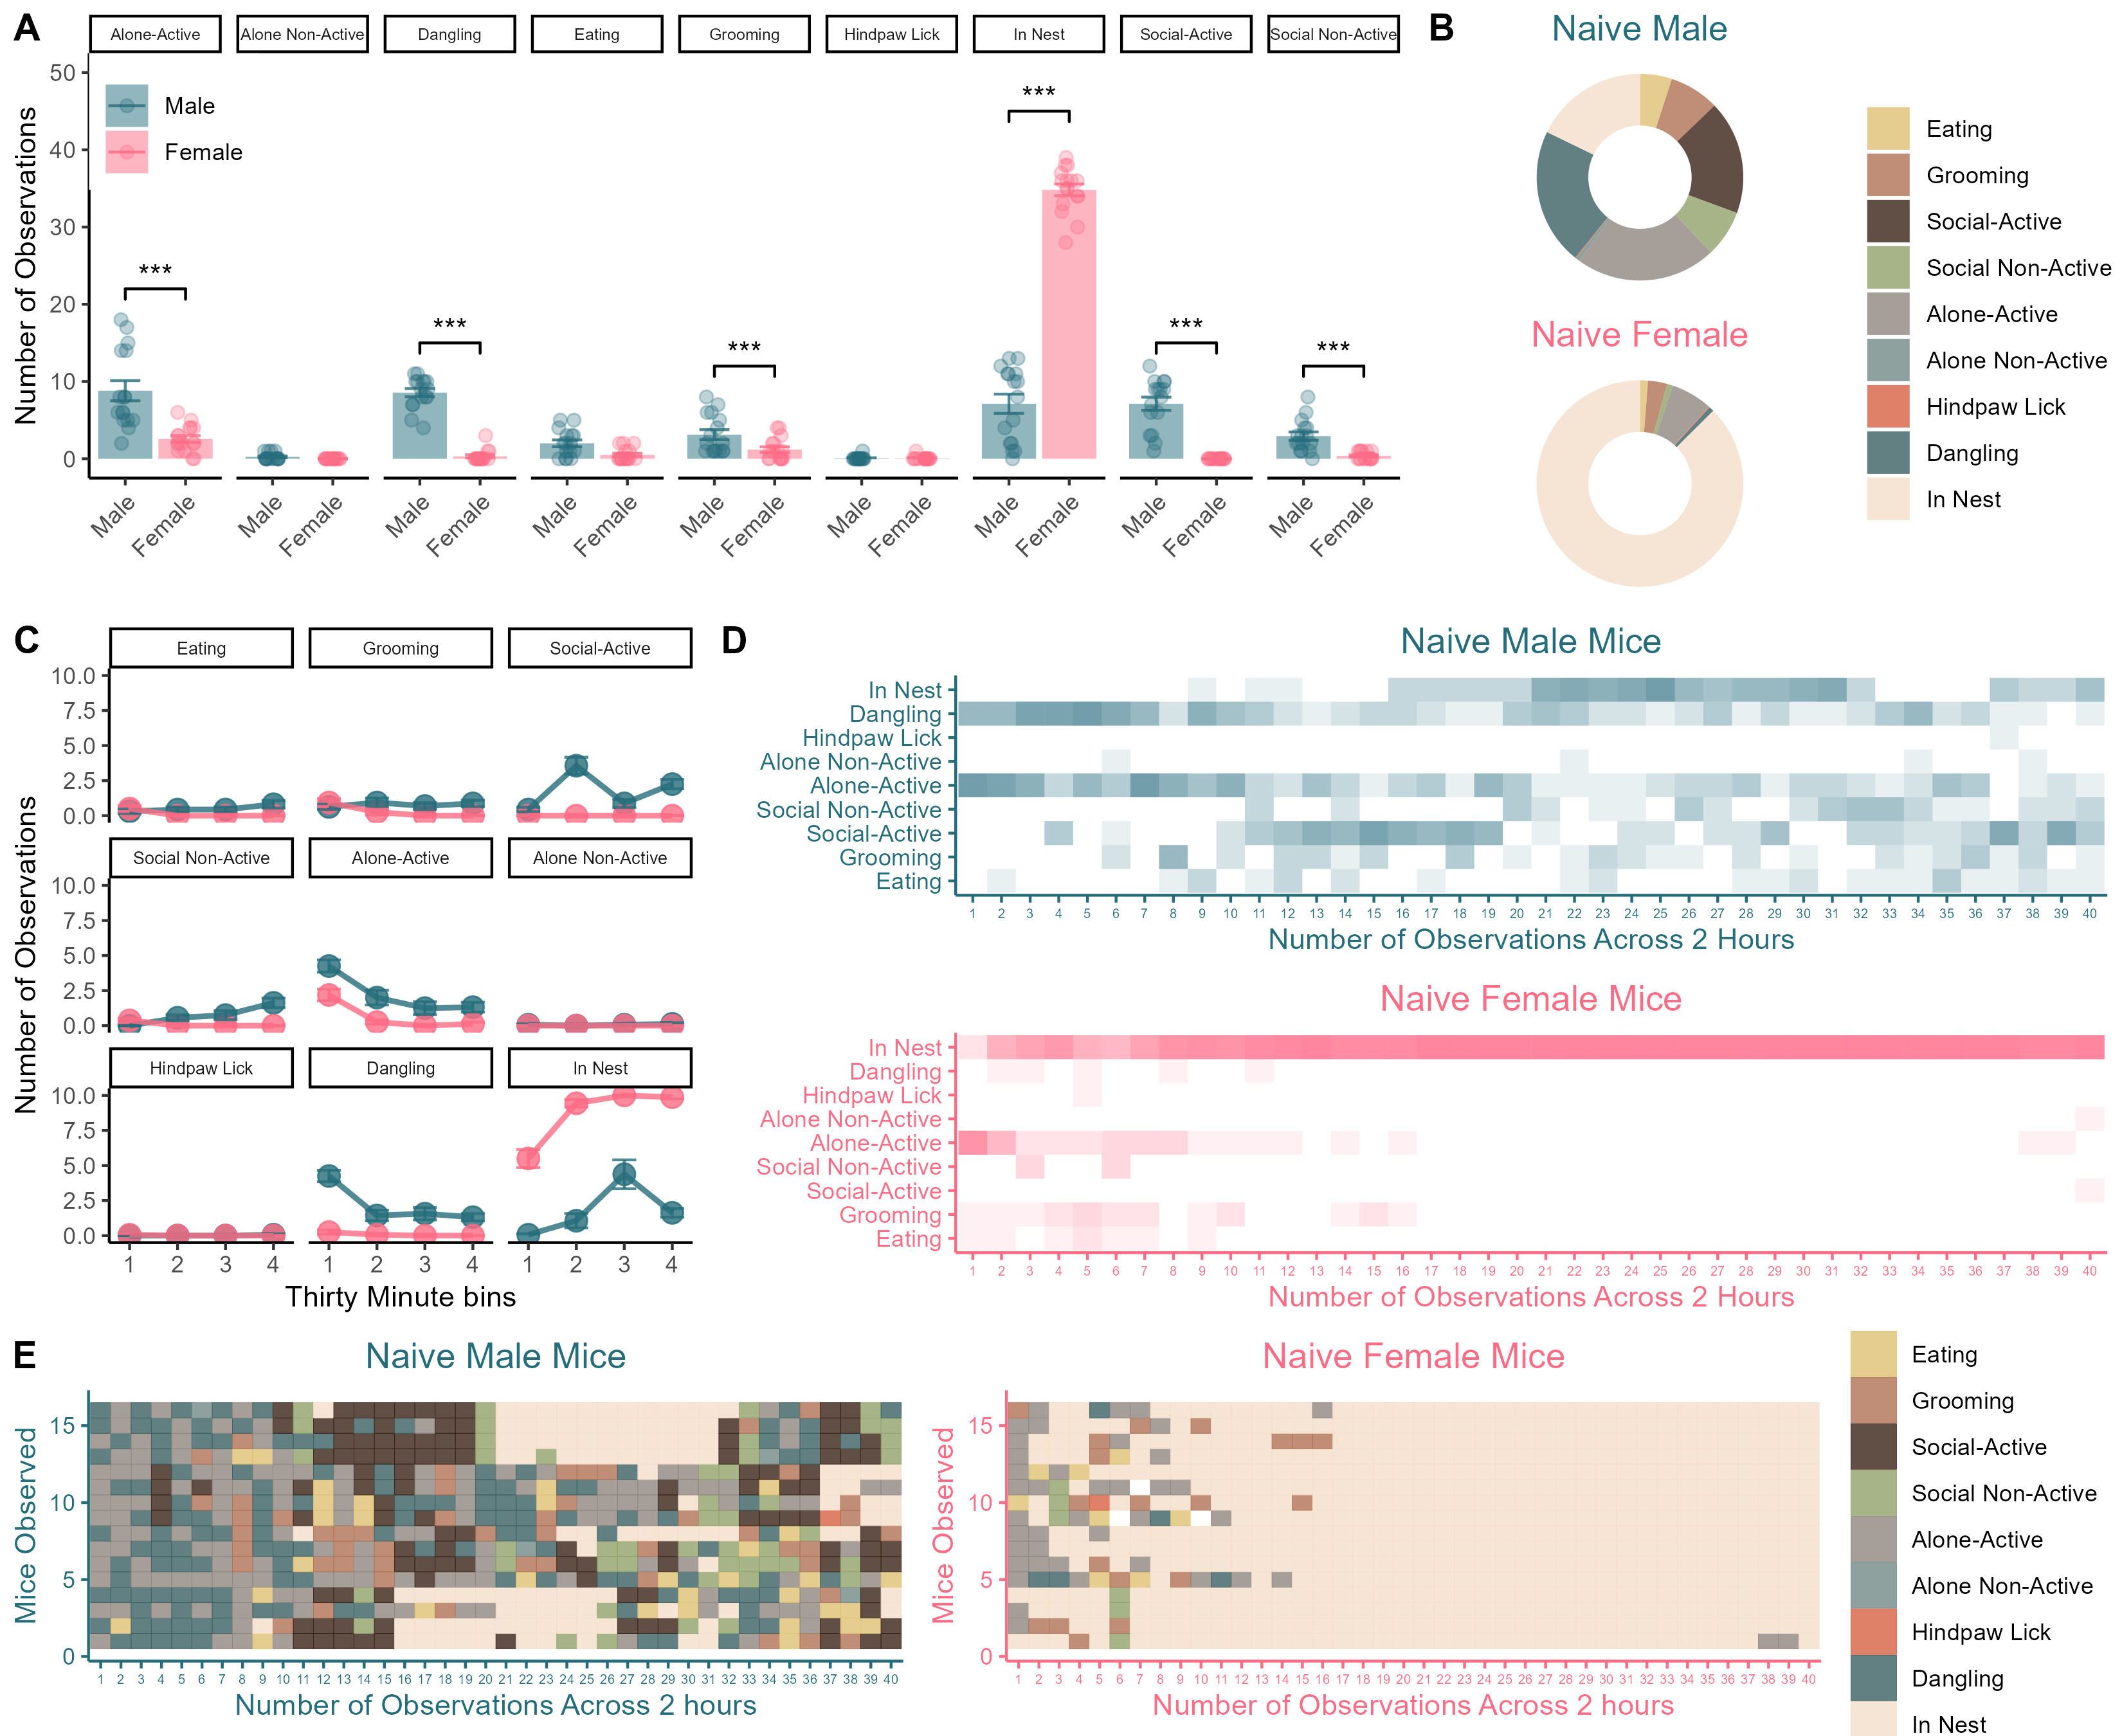
\includegraphics[width=45.83in]{Figs/S1_MvF_Homecage} \end{center}

\textbf{Figure S1.} \emph{Sex differences in basal homecage behavior.} (A) total quantification of observations across the two hour session expressed as mean value +/- SEM. (B) Donut charts showcasing the frequency of behaviors observed for males and females. (C) Line charts showing changes across the session divided into 4x30 minute bins. (D and E) are qualitative representations of the distribution of behaviors observed across the 40 timepoints.

\hypertarget{statistics-2}{%
\section*{Statistics}\label{statistics-2}}
\addcontentsline{toc}{section}{Statistics}

\begin{Shaded}
\begin{Highlighting}[]
\DocumentationTok{\#\# MANOVA on SEX in the Naives: }
\NormalTok{a }\OtherTok{\textless{}{-}}\NormalTok{ m\_male\_data }\SpecialCharTok{\%\textgreater{}\%}
  \FunctionTok{group\_by}\NormalTok{(ID,Sex,value) }\SpecialCharTok{\%\textgreater{}\%}
  \FunctionTok{summarise}\NormalTok{(}
    \AttributeTok{my\_count=}\FunctionTok{n}\NormalTok{()}
\NormalTok{  ) }
  
\NormalTok{b }\OtherTok{\textless{}{-}} \FunctionTok{dcast}\NormalTok{(a,ID}\SpecialCharTok{+}\NormalTok{Sex}\SpecialCharTok{\textasciitilde{}}\NormalTok{value,}\AttributeTok{value.var =} \StringTok{"my\_count"}\NormalTok{)}

\NormalTok{b }\OtherTok{\textless{}{-}}\NormalTok{ b }\SpecialCharTok{\%\textgreater{}\%} 
  \FunctionTok{mutate\_at}\NormalTok{(}\FunctionTok{c}\NormalTok{(}\DecValTok{3}\SpecialCharTok{:}\DecValTok{12}\NormalTok{), }\SpecialCharTok{\textasciitilde{}}\FunctionTok{replace}\NormalTok{(., }\FunctionTok{is.na}\NormalTok{(.), }\DecValTok{0}\NormalTok{))}

\NormalTok{fit }\OtherTok{\textless{}{-}} \FunctionTok{manova}\NormalTok{(}\FunctionTok{cbind}\NormalTok{(Grooming,}\StringTok{\textasciigrave{}}\AttributeTok{Social{-}Active}\StringTok{\textasciigrave{}}\NormalTok{,}\StringTok{\textasciigrave{}}\AttributeTok{Social Non{-}Active}\StringTok{\textasciigrave{}}\NormalTok{,}\StringTok{\textasciigrave{}}\AttributeTok{Alone{-}Active}\StringTok{\textasciigrave{}}\NormalTok{,}\StringTok{\textasciigrave{}}\AttributeTok{Alone Non{-}Active}\StringTok{\textasciigrave{}}\NormalTok{,}\StringTok{\textasciigrave{}}\AttributeTok{Hindpaw Lick}\StringTok{\textasciigrave{}}\NormalTok{,}\StringTok{\textasciigrave{}}\AttributeTok{Dangling}\StringTok{\textasciigrave{}}\NormalTok{,}\StringTok{\textasciigrave{}}\AttributeTok{In Nest}\StringTok{\textasciigrave{}}\NormalTok{) }\SpecialCharTok{\textasciitilde{}}\NormalTok{ Sex, }\AttributeTok{data=}\NormalTok{b)}
\FunctionTok{summary}\NormalTok{(fit)}
\end{Highlighting}
\end{Shaded}

\begin{verbatim}
##           Df Pillai approx F num Df den Df                Pr(>F)    
## Sex        1  0.974   107.69      8     23 0.0000000000000002247 ***
## Residuals 30                                                        
## ---
## Signif. codes:  0 '***' 0.001 '**' 0.01 '*' 0.05 '.' 0.1 ' ' 1
\end{verbatim}

\begin{Shaded}
\begin{Highlighting}[]
\CommentTok{\# Because the omnibus test (above) is significant, follow up by running one{-}way ANOVAs for each behavior. }
\DocumentationTok{\#\# Bonferroni correct these only if forced}
\FunctionTok{summary.aov}\NormalTok{(fit)}
\end{Highlighting}
\end{Shaded}

\begin{verbatim}
##  Response Grooming :
##             Df  Sum Sq Mean Sq F value  Pr(>F)  
## Sex          1  30.031 30.0312  7.2547 0.01146 *
## Residuals   30 124.187  4.1396                  
## ---
## Signif. codes:  0 '***' 0.001 '**' 0.01 '*' 0.05 '.' 0.1 ' ' 1
## 
##  Response Social-Active :
##             Df Sum Sq Mean Sq F value         Pr(>F)    
## Sex          1 406.13  406.13  74.405 0.000000001271 ***
## Residuals   30 163.75    5.46                           
## ---
## Signif. codes:  0 '***' 0.001 '**' 0.01 '*' 0.05 '.' 0.1 ' ' 1
## 
##  Response Social Non-Active :
##             Df Sum Sq Mean Sq F value     Pr(>F)    
## Sex          1 52.531  52.531  22.944 0.00004214 ***
## Residuals   30 68.687   2.290                       
## ---
## Signif. codes:  0 '***' 0.001 '**' 0.01 '*' 0.05 '.' 0.1 ' ' 1
## 
##  Response Alone-Active :
##             Df Sum Sq Mean Sq F value     Pr(>F)    
## Sex          1 312.50 312.500  21.988 0.00005597 ***
## Residuals   30 426.38  14.213                       
## ---
## Signif. codes:  0 '***' 0.001 '**' 0.01 '*' 0.05 '.' 0.1 ' ' 1
## 
##  Response Alone Non-Active :
##             Df Sum Sq Mean Sq F value  Pr(>F)  
## Sex          1    0.5     0.5       5 0.03294 *
## Residuals   30    3.0     0.1                  
## ---
## Signif. codes:  0 '***' 0.001 '**' 0.01 '*' 0.05 '.' 0.1 ' ' 1
## 
##  Response Hindpaw Lick :
##             Df Sum Sq Mean Sq F value Pr(>F)
## Sex          1  0.000  0.0000       0      1
## Residuals   30  1.875  0.0625               
## 
##  Response Dangling :
##             Df Sum Sq Mean Sq F value               Pr(>F)    
## Sex          1 544.50  544.50  228.86 0.000000000000001398 ***
## Residuals   30  71.38    2.38                                 
## ---
## Signif. codes:  0 '***' 0.001 '**' 0.01 '*' 0.05 '.' 0.1 ' ' 1
## 
##  Response In Nest :
##             Df Sum Sq Mean Sq F value                Pr(>F)    
## Sex          1 6132.8  6132.8  384.75 < 0.00000000000000022 ***
## Residuals   30  478.2    15.9                                  
## ---
## Signif. codes:  0 '***' 0.001 '**' 0.01 '*' 0.05 '.' 0.1 ' ' 1
\end{verbatim}

\begin{itemize}
\tightlist
\item
  Females spent less time grooming (F(1,30) = 7.25, p = 0.01)
\item
  Less socially active (F(1,30) = 74.405, p \textless{} 0.001)
\item
  Less socially non-active (F(1,30) = 22.94, p \textless{} 0.001)
\item
  Less alone active (F(1,30) = 21.988, p \textless{} 0.001)
\item
  Less alone non-active (F(1,30) = 5, p = 0.032)
\item
  Less dangling (F(1,30) = 228.86, p \textless{} 0.001)
\end{itemize}

\ldots{} Because they spend so much more time than males in the nest (F(1,30) = 384.75, p \textless{} 0.001)

\hypertarget{supplemental-figure-2---sex-differences-in-cfa-hypersensitivity-recovery}{%
\chapter*{Supplemental Figure 2 - Sex differences in CFA Hypersensitivity \& Recovery}\label{supplemental-figure-2---sex-differences-in-cfa-hypersensitivity-recovery}}
\addcontentsline{toc}{chapter}{Supplemental Figure 2 - Sex differences in CFA Hypersensitivity \& Recovery}

\begin{center}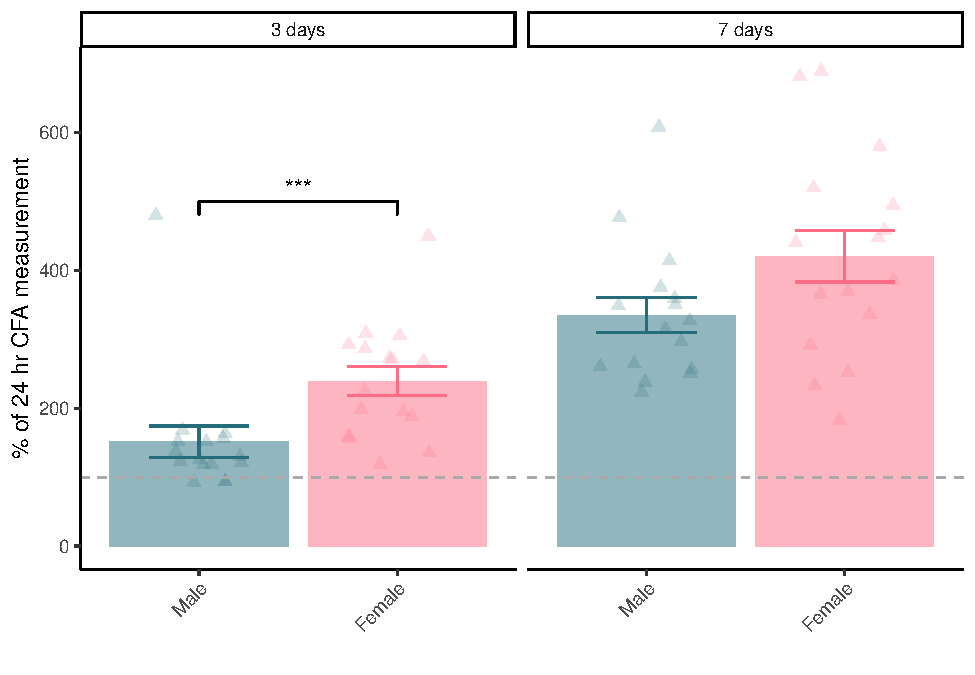
\includegraphics{_main_files/figure-latex/unnamed-chunk-53-1} \end{center}

\hypertarget{published-image-6}{%
\section*{Published Image}\label{published-image-6}}
\addcontentsline{toc}{section}{Published Image}

\begin{center}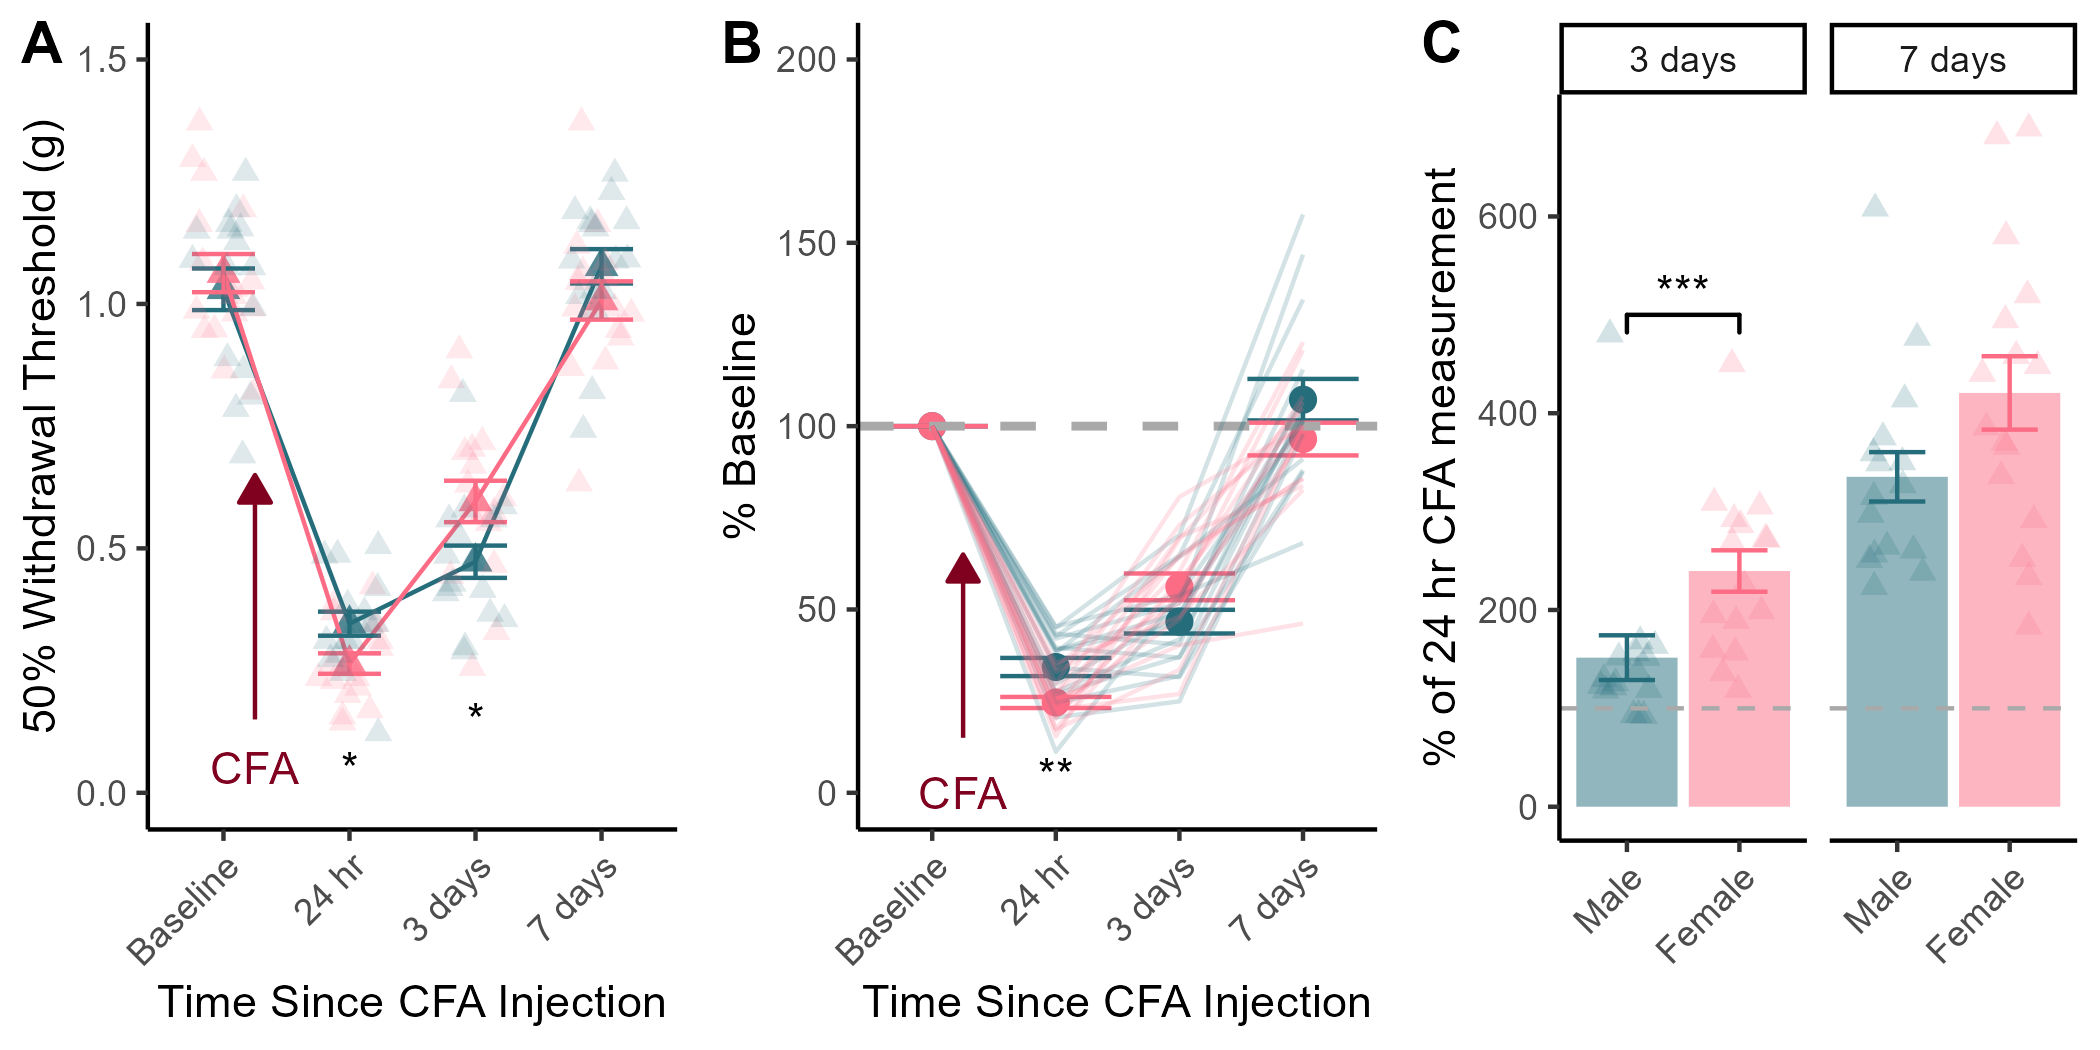
\includegraphics[width=29.17in]{Figs/S2_MvF_CFA} \end{center}

\textbf{Figure S2.} \emph{Sex differences in hypersensitivity caused by CFA injection.} (A) Female mice exhibit more sensitivity than males 24 hours after CFA, but less sensitivity than males 3 days post administration. (B) CFA induced more robust sensitivity in female mice than males at the 24 hour post injection timepoint, relative to the individual baseline measurements. (C) Female mice exhibited a greater resolution of sensitivity than did males between the first two post CFA VF measurements. Data expressed as mean value +/- SEM, *** indicates p \textless{} 0.001, ** indicates p \textless{} 0.01, * indicates p \textless{} 0.05.

\hypertarget{statistics-3}{%
\section*{Statistics}\label{statistics-3}}
\addcontentsline{toc}{section}{Statistics}

\begin{Shaded}
\begin{Highlighting}[]
\CommentTok{\# Raw VF values {-} stats}
\NormalTok{a }\OtherTok{\textless{}{-}}\NormalTok{ CFAs\_left }\SpecialCharTok{\%\textgreater{}\%}
  \FunctionTok{melt}\NormalTok{(}\AttributeTok{id.vars=}\FunctionTok{c}\NormalTok{(}\StringTok{"ID"}\NormalTok{,}\StringTok{"Sex"}\NormalTok{,}\StringTok{"CFA"}\NormalTok{)) }

\NormalTok{b }\OtherTok{\textless{}{-}}\NormalTok{ a }\SpecialCharTok{\%\textgreater{}\%}
  \FunctionTok{group\_by}\NormalTok{(variable) }\SpecialCharTok{\%\textgreater{}\%}
  \FunctionTok{pairwise\_t\_test}\NormalTok{(value}\SpecialCharTok{\textasciitilde{}}\NormalTok{Sex)}

\FunctionTok{tt}\NormalTok{(b)}
\end{Highlighting}
\end{Shaded}

\begin{table}
\centering
\begin{tblr}[         %% tabularray outer open
]                     %% tabularray outer close
{                     %% tabularray inner open
colspec={Q[]Q[]Q[]Q[]Q[]Q[]Q[]Q[]Q[]Q[]},
}                     %% tabularray inner close
\toprule
variable & .y. & group1 & group2 & n1 & n2 & p & p.signif & p.adj & p.adj.signif \\ \midrule %% TinyTableHeader
Baseline & value & Male & Female & 16 & 16 & 0.5710 & ns & 0.5710 & ns \\
24 hr    & value & Male & Female & 16 & 16 & 0.0170 & *  & 0.0170 & *  \\
3 days   & value & Male & Female & 16 & 16 & 0.0288 & *  & 0.0288 & *  \\
7 days   & value & Male & Female & 16 & 16 & 0.1940 & ns & 0.1940 & ns \\
\bottomrule
\end{tblr}
\end{table}

\begin{itemize}
\tightlist
\item
  There were no sex differences in basal paw withdrawal thresholds (p = 0.57)
\item
  24 hours post CFA, female mice had lower paw withdrawal thresholds than males(p - 0.017)
\item
  3 days post CFA, female mice had higher paw withdrawal thresholds than females(p=0.028)
\end{itemize}

\begin{Shaded}
\begin{Highlighting}[]
\CommentTok{\# \% Baseline Stats}
\NormalTok{a }\OtherTok{\textless{}{-}}\NormalTok{ CFAs\_left }\SpecialCharTok{\%\textgreater{}\%}
  \FunctionTok{mutate}\NormalTok{(}\StringTok{\textasciigrave{}}\AttributeTok{24 hr}\StringTok{\textasciigrave{}} \OtherTok{=}\NormalTok{ (}\StringTok{\textasciigrave{}}\AttributeTok{24 hr}\StringTok{\textasciigrave{}} \SpecialCharTok{/} \StringTok{\textasciigrave{}}\AttributeTok{Baseline}\StringTok{\textasciigrave{}}\NormalTok{) }\SpecialCharTok{*} \DecValTok{100}\NormalTok{) }\SpecialCharTok{\%\textgreater{}\%}
  \FunctionTok{mutate}\NormalTok{(}\StringTok{\textasciigrave{}}\AttributeTok{3 days}\StringTok{\textasciigrave{}} \OtherTok{=}\NormalTok{ (}\StringTok{\textasciigrave{}}\AttributeTok{3 days}\StringTok{\textasciigrave{}} \SpecialCharTok{/} \StringTok{\textasciigrave{}}\AttributeTok{Baseline}\StringTok{\textasciigrave{}}\NormalTok{) }\SpecialCharTok{*} \DecValTok{100}\NormalTok{) }\SpecialCharTok{\%\textgreater{}\%}
  \FunctionTok{mutate}\NormalTok{(}\StringTok{\textasciigrave{}}\AttributeTok{7 days}\StringTok{\textasciigrave{}} \OtherTok{=}\NormalTok{ (}\StringTok{\textasciigrave{}}\AttributeTok{7 days}\StringTok{\textasciigrave{}} \SpecialCharTok{/} \StringTok{\textasciigrave{}}\AttributeTok{Baseline}\StringTok{\textasciigrave{}}\NormalTok{) }\SpecialCharTok{*} \DecValTok{100}\NormalTok{) }\SpecialCharTok{\%\textgreater{}\%}
  \FunctionTok{mutate}\NormalTok{(}\AttributeTok{Baseline =} \DecValTok{100}\NormalTok{) }\SpecialCharTok{\%\textgreater{}\%}
  \FunctionTok{melt}\NormalTok{(}\AttributeTok{id.vars=}\FunctionTok{c}\NormalTok{(}\StringTok{"ID"}\NormalTok{,}\StringTok{"Sex"}\NormalTok{,}\StringTok{"CFA"}\NormalTok{)) }\SpecialCharTok{\%\textgreater{}\%}
  \FunctionTok{filter}\NormalTok{(CFA }\SpecialCharTok{==} \StringTok{"CFA"}\NormalTok{)}

\NormalTok{b }\OtherTok{\textless{}{-}}\NormalTok{ a }\SpecialCharTok{\%\textgreater{}\%} 
  \FunctionTok{group\_by}\NormalTok{(variable) }\SpecialCharTok{\%\textgreater{}\%}
  \FunctionTok{pairwise\_t\_test}\NormalTok{(value}\SpecialCharTok{\textasciitilde{}}\NormalTok{Sex)}

\FunctionTok{tt}\NormalTok{(b)}
\end{Highlighting}
\end{Shaded}

\begin{table}
\centering
\begin{tblr}[         %% tabularray outer open
]                     %% tabularray outer close
{                     %% tabularray inner open
colspec={Q[]Q[]Q[]Q[]Q[]Q[]Q[]Q[]Q[]Q[]},
}                     %% tabularray inner close
\toprule
variable & .y. & group1 & group2 & n1 & n2 & p & p.signif & p.adj & p.adj.signif \\ \midrule %% TinyTableHeader
24 hr  & value & Male & Female & 16 & 16 & 0.0023 & ** & 0.0023 & ** \\
3 days & value & Male & Female & 16 & 16 & 0.0606 & ns & 0.0606 & ns \\
7 days & value & Male & Female & 16 & 16 & 0.1470 & ns & 0.1470 & ns \\
\bottomrule
\end{tblr}
\end{table}

\begin{itemize}
\item
  at the 24 hour timepoint, the \% baseline value for female CFA-injected mice was lower than for CFA-injected males (p = 0.0023)
\item
  Three and Seven days post-injection, there was no sex difference in the \% baseline (p = 0.061, p = 0.15, respectively).
\end{itemize}

These findings suggest that there may be sex differences in the timecourese of recovery after CFA injection in our model. Females initially exhibit more robust sensitivity at the site of CFA injection compared to males, but exhibit more recovery than males during the following 48 hour interval.

\hypertarget{supplemental-figure-3---sex-differences-in-hyperalgesic-priming}{%
\chapter*{Supplemental Figure 3 - Sex Differences in Hyperalgesic Priming}\label{supplemental-figure-3---sex-differences-in-hyperalgesic-priming}}
\addcontentsline{toc}{chapter}{Supplemental Figure 3 - Sex Differences in Hyperalgesic Priming}

\begin{itemize}
\item
  Priming was \textbf{induced} by CFA.
\item
  \textbf{Expression} of priming was elicited by 100ng PGE-2 administration at the site of previous injury.
\end{itemize}

\hypertarget{published-image-7}{%
\section*{Published Image}\label{published-image-7}}
\addcontentsline{toc}{section}{Published Image}

\begin{center}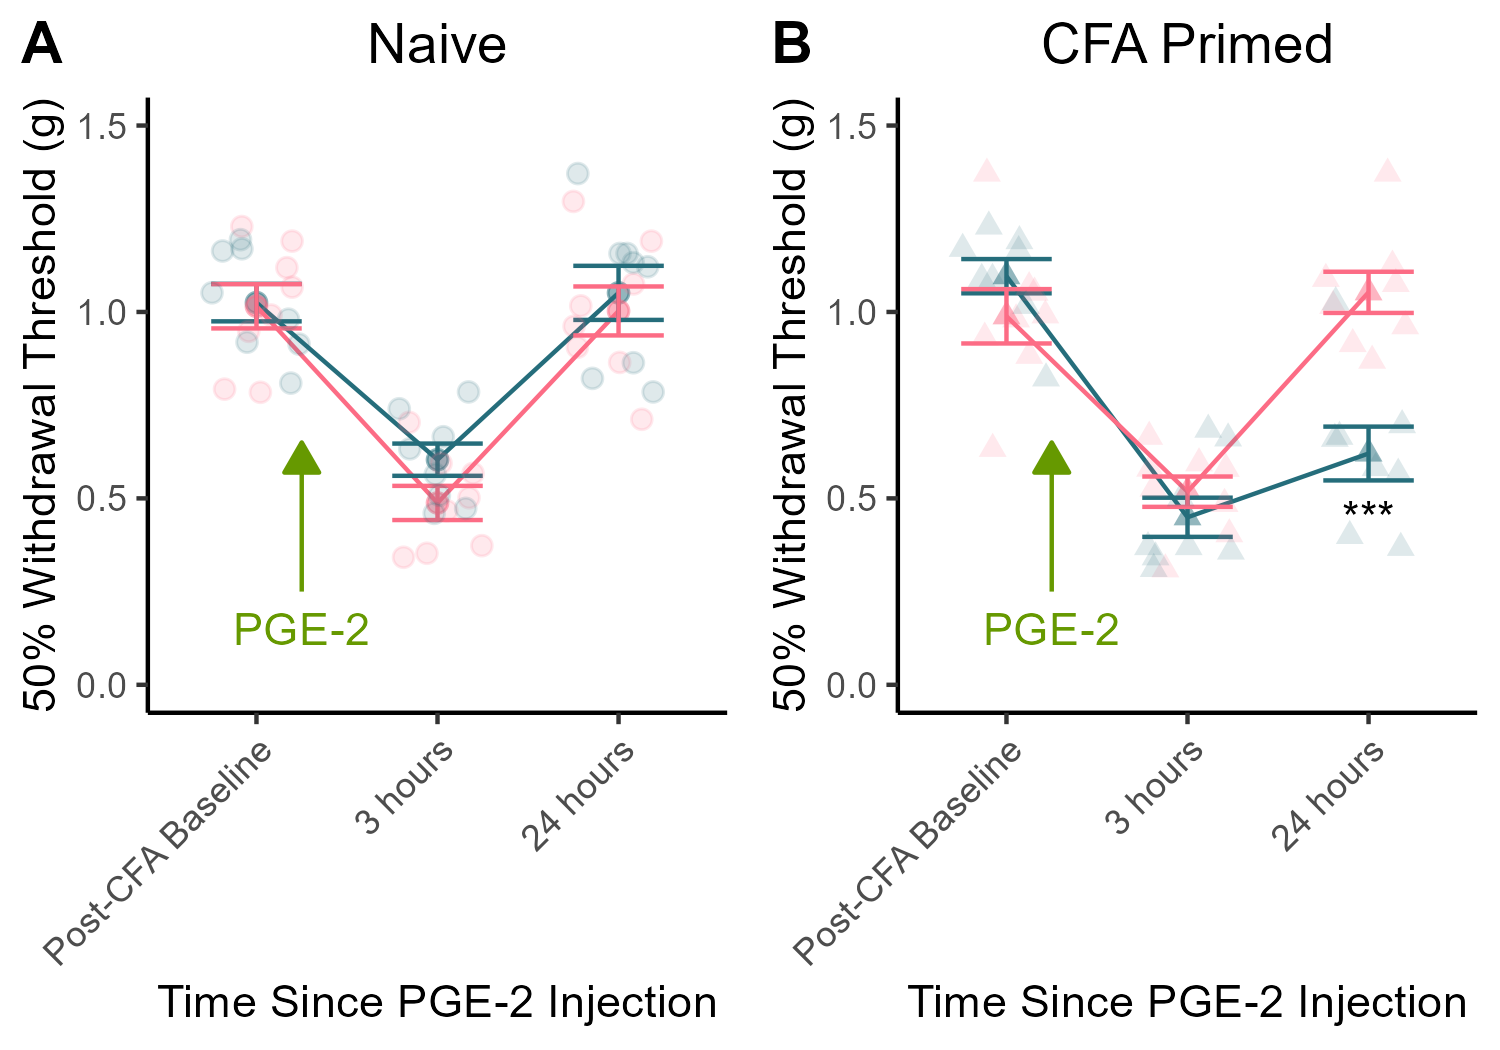
\includegraphics[width=20.83in]{Figs/S3_MvF_PGE2} \end{center}

\textbf{Figure S3.} \emph{Sex differences in PGE-2-induced expression of Hyperalgesic priming.} (A) There is no sex difference in the magnitude of mechanical sensitivity induced by PGE-2 administration in naive mice. (B) Among CFA-primed mice, males exhibit more sensitivity than females 24 hours post PGE-2 administration. Data expressed as mean value +/- SEM, *** indicates p \textless{} 0.001.

\hypertarget{statistics-4}{%
\section*{Statistics}\label{statistics-4}}
\addcontentsline{toc}{section}{Statistics}

\begin{Shaded}
\begin{Highlighting}[]
\NormalTok{a }\OtherTok{\textless{}{-}}\NormalTok{ m\_Left[m\_Left}\SpecialCharTok{$}\NormalTok{CFA }\SpecialCharTok{==} \StringTok{"CFA"}\NormalTok{, ]}

\NormalTok{b }\OtherTok{\textless{}{-}}\NormalTok{ m\_Left }\SpecialCharTok{\%\textgreater{}\%}
  \FunctionTok{filter}\NormalTok{(CFA }\SpecialCharTok{==} \StringTok{"CFA"}\NormalTok{) }\SpecialCharTok{\%\textgreater{}\%}
  \FunctionTok{group\_by}\NormalTok{(variable) }\SpecialCharTok{\%\textgreater{}\%}
  \FunctionTok{pairwise\_t\_test}\NormalTok{(value}\SpecialCharTok{\textasciitilde{}}\NormalTok{Sex)}

\FunctionTok{tt}\NormalTok{(b)}
\end{Highlighting}
\end{Shaded}

\begin{table}
\centering
\begin{tblr}[         %% tabularray outer open
]                     %% tabularray outer close
{                     %% tabularray inner open
colspec={Q[]Q[]Q[]Q[]Q[]Q[]Q[]Q[]Q[]Q[]},
}                     %% tabularray inner close
\toprule
variable & .y. & group1 & group2 & n1 & n2 & p & p.signif & p.adj & p.adj.signif \\ \midrule %% TinyTableHeader
Post-CFA Baseline & value & Male & Female & 8 & 8 & 0.232000 & ns  & 0.232000 & ns  \\
3 hours           & value & Male & Female & 8 & 8 & 0.319000 & ns  & 0.319000 & ns  \\
24 hours          & value & Male & Female & 8 & 8 & 0.000306 & *** & 0.000306 & *** \\
\bottomrule
\end{tblr}
\end{table}

\begin{itemize}
\tightlist
\item
  24 hours after PGE-2 administration, CFA-primed males exhibit ongoing hypersensitivity, whereas CFA-primed females do not.
\end{itemize}

\hypertarget{supplemental-figure-4---sex-differences-in-shock-induced-sensitivity}{%
\chapter*{Supplemental Figure 4 - Sex Differences in Shock-Induced Sensitivity}\label{supplemental-figure-4---sex-differences-in-shock-induced-sensitivity}}
\addcontentsline{toc}{chapter}{Supplemental Figure 4 - Sex Differences in Shock-Induced Sensitivity}

\hypertarget{published-image-8}{%
\section*{Published Image}\label{published-image-8}}
\addcontentsline{toc}{section}{Published Image}

\begin{center}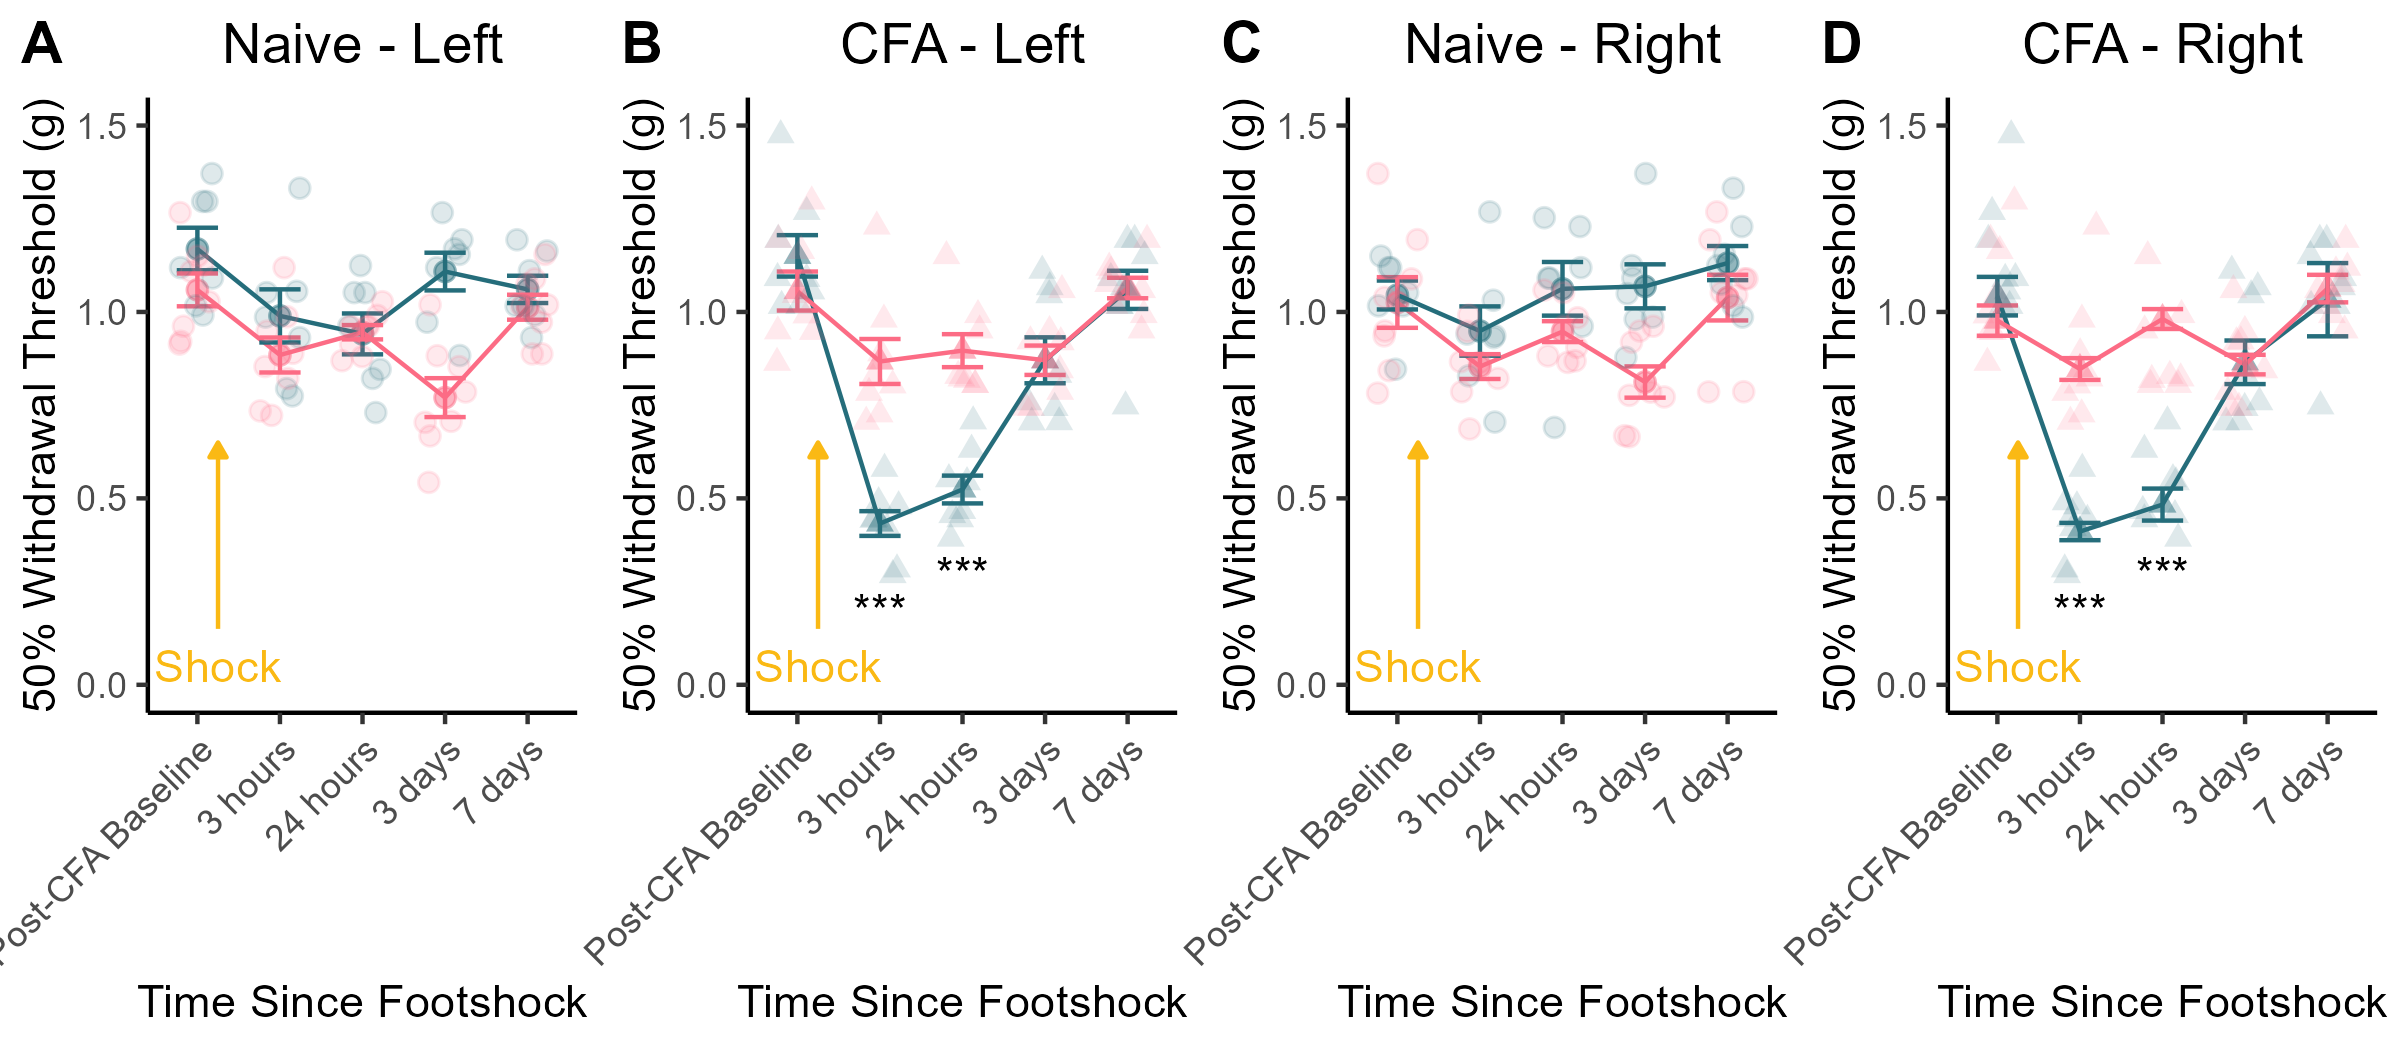
\includegraphics[width=33.33in]{Figs/S4_Shock} \end{center}

\textbf{Figure S4.} \emph{Sex differences in footshock-induced expression of hyperalgesic priming.} (A) There was no sex difference in the magnitude of footshock-induced mechanical sensitivity among nive mice. (B) CFA-primed mice males exhibited expression of hyperalgesic priming at the site of previous injury whereas female CFA-primed mice did not. (C) Naive mice did not express footshock induced changes in sensitivity, but (D) male CFA-primed mice exhibited expression of hyperalgesic priming after footshock in their right paw as well (which had not been injured by CFA). Data expressed as mean value +/- SEM, *** indicates p \textless{} 0.001.

\hypertarget{statistics-5}{%
\section*{Statistics}\label{statistics-5}}
\addcontentsline{toc}{section}{Statistics}

\begin{Shaded}
\begin{Highlighting}[]
\DocumentationTok{\#\# CFA{-}primed: Left Paws}

\NormalTok{a }\OtherTok{\textless{}{-}}\NormalTok{ Left\_data }\SpecialCharTok{\%\textgreater{}\%}
  \FunctionTok{melt}\NormalTok{(}\AttributeTok{id.vars =} \FunctionTok{c}\NormalTok{(}\StringTok{"ID"}\NormalTok{,}\StringTok{"Sex"}\NormalTok{,}\StringTok{"CFA"}\NormalTok{)) }\SpecialCharTok{\%\textgreater{}\%} 
  \FunctionTok{filter}\NormalTok{(CFA }\SpecialCharTok{==} \StringTok{"CFA"}\NormalTok{)}

\NormalTok{b }\OtherTok{\textless{}{-}} \FunctionTok{aov}\NormalTok{(}\AttributeTok{data=}\NormalTok{a,value}\SpecialCharTok{\textasciitilde{}}\NormalTok{variable}\SpecialCharTok{*}\NormalTok{Sex)}
\FunctionTok{summary}\NormalTok{(b)}
\end{Highlighting}
\end{Shaded}

\begin{verbatim}
##              Df Sum Sq Mean Sq F value               Pr(>F)    
## variable      4 2.6377  0.6594   36.44 < 0.0000000000000002 ***
## Sex           1 0.4122  0.4122   22.78         0.0000096220 ***
## variable:Sex  4 0.9339  0.2335   12.90         0.0000000637 ***
## Residuals    70 1.2666  0.0181                                 
## ---
## Signif. codes:  0 '***' 0.001 '**' 0.01 '*' 0.05 '.' 0.1 ' ' 1
\end{verbatim}

\begin{Shaded}
\begin{Highlighting}[]
\NormalTok{c }\OtherTok{\textless{}{-}}\NormalTok{ a }\SpecialCharTok{\%\textgreater{}\%}
  \FunctionTok{group\_by}\NormalTok{(variable) }\SpecialCharTok{\%\textgreater{}\%}
  \FunctionTok{pairwise\_t\_test}\NormalTok{(value}\SpecialCharTok{\textasciitilde{}}\NormalTok{Sex)}

\FunctionTok{tt}\NormalTok{(c)}
\end{Highlighting}
\end{Shaded}

\begin{table}
\centering
\begin{tblr}[         %% tabularray outer open
]                     %% tabularray outer close
{                     %% tabularray inner open
colspec={Q[]Q[]Q[]Q[]Q[]Q[]Q[]Q[]Q[]Q[]},
}                     %% tabularray inner close
\toprule
variable & .y. & group1 & group2 & n1 & n2 & p & p.signif & p.adj & p.adj.signif \\ \midrule %% TinyTableHeader
Post-CFA Baseline & value & Male & Female & 8 & 8 & 0.2360000 & ns   & 0.2360000 & ns   \\
3 hours           & value & Male & Female & 8 & 8 & 0.0000190 & **** & 0.0000190 & **** \\
24 hours          & value & Male & Female & 8 & 8 & 0.0000155 & **** & 0.0000155 & **** \\
3 days            & value & Male & Female & 8 & 8 & 0.9980000 & ns   & 0.9980000 & ns   \\
7 days            & value & Male & Female & 8 & 8 & 0.9330000 & ns   & 0.9330000 & ns   \\
\bottomrule
\end{tblr}
\end{table}

\begin{itemize}
\item
  Both Three and 24 hours after footshock, CFA-primed males exhibit more hypersensitvity than CFA-primed females.
\item
  There are no group differences at baseline, 3 days post shock, or 7 days post shock.
\end{itemize}

\begin{Shaded}
\begin{Highlighting}[]
\DocumentationTok{\#\# CFA{-}primed: Right Paws}

\NormalTok{a }\OtherTok{\textless{}{-}}\NormalTok{ Right\_data }\SpecialCharTok{\%\textgreater{}\%}
  \FunctionTok{melt}\NormalTok{(}\AttributeTok{id.vars =} \FunctionTok{c}\NormalTok{(}\StringTok{"ID"}\NormalTok{,}\StringTok{"Sex"}\NormalTok{,}\StringTok{"CFA"}\NormalTok{)) }\SpecialCharTok{\%\textgreater{}\%} 
  \FunctionTok{filter}\NormalTok{(CFA }\SpecialCharTok{==} \StringTok{"CFA"}\NormalTok{)}

\NormalTok{b }\OtherTok{\textless{}{-}} \FunctionTok{aov}\NormalTok{(}\AttributeTok{data=}\NormalTok{a,value}\SpecialCharTok{\textasciitilde{}}\NormalTok{variable}\SpecialCharTok{*}\NormalTok{Sex)}
\FunctionTok{summary}\NormalTok{(b)}
\end{Highlighting}
\end{Shaded}

\begin{verbatim}
##              Df Sum Sq Mean Sq F value            Pr(>F)    
## variable      4 2.0363  0.5091   27.21 0.000000000000123 ***
## Sex           1 0.6361  0.6361   34.00 0.000000155168408 ***
## variable:Sex  4 1.1357  0.2839   15.18 0.000000005554703 ***
## Residuals    70 1.3095  0.0187                              
## ---
## Signif. codes:  0 '***' 0.001 '**' 0.01 '*' 0.05 '.' 0.1 ' ' 1
\end{verbatim}

\begin{Shaded}
\begin{Highlighting}[]
\NormalTok{c }\OtherTok{\textless{}{-}}\NormalTok{ a }\SpecialCharTok{\%\textgreater{}\%}
  \FunctionTok{group\_by}\NormalTok{(variable) }\SpecialCharTok{\%\textgreater{}\%}
  \FunctionTok{pairwise\_t\_test}\NormalTok{(value}\SpecialCharTok{\textasciitilde{}}\NormalTok{Sex)}

\FunctionTok{tt}\NormalTok{(c)}
\end{Highlighting}
\end{Shaded}

\begin{table}
\centering
\begin{tblr}[         %% tabularray outer open
]                     %% tabularray outer close
{                     %% tabularray inner open
colspec={Q[]Q[]Q[]Q[]Q[]Q[]Q[]Q[]Q[]Q[]},
}                     %% tabularray inner close
\toprule
variable & .y. & group1 & group2 & n1 & n2 & p & p.signif & p.adj & p.adj.signif \\ \midrule %% TinyTableHeader
Post-CFA Baseline & value & Male & Female & 8 & 8 & 0.3350000000 & ns   & 0.3350000000 & ns   \\
3 hours           & value & Male & Female & 8 & 8 & 0.0000000132 & **** & 0.0000000132 & **** \\
24 hours          & value & Male & Female & 8 & 8 & 0.0000001120 & **** & 0.0000001120 & **** \\
3 days            & value & Male & Female & 8 & 8 & 0.9250000000 & ns   & 0.9250000000 & ns   \\
7 days            & value & Male & Female & 8 & 8 & 0.7800000000 & ns   & 0.7800000000 & ns   \\
\bottomrule
\end{tblr}
\end{table}

\begin{itemize}
\item
  Both Three and 24 hours after footshock, CFA-primed males exhibit more hypersensitvity than CFA-primed females.
\item
  There are no group differences at baseline, 3 days post shock, or 7 days post shock.
\end{itemize}

Similar statistical results for the left and right hind paws indicate that the expression of hyperalgesic priming is not limited to the site of previous injury in male mice.

  \bibliography{book.bib,packages.bib}

\end{document}
